% concatenated from arXiv.tex, preamble.tex


\documentclass[journal]{IEEEtran}
%\addtolength{\topmargin}{9mm}

%\documentclass[10pt, journal,letterpaper, onecolumn]{IEEEtran}

%% depending on your installation, you may wish to adjust the top margin:
%\addtolength{\topmargin}{9mm}
%\include{preamble}
%%%%%%
%% Packages:
%% Some useful packages (and compatibility issues with the IEEE format)
%% are pointed out at the very end of this template source file (they are 
%% taken verbatim out of bare_conf.tex by Michael Shell).
%
% *** Do not adjust lengths that control margins, column widths, etc. ***
% *** Do not use packages that alter fonts (such as pslatex).         ***
%
\usepackage[utf8]{inputenc} 
\usepackage[T1]{fontenc}
\usepackage{url}
\usepackage{ifthen}
\usepackage{enumitem}

\usepackage{tikz}
\usetikzlibrary{arrows.meta, positioning}
%\usepackage{cite}
%\usepackage[cmex10]{amsmath} % Use the [cmex10] option to ensure complicance
                             % with IEEE Xplore (see bare_conf.tex)

%% Please note that the amsthm package must not be loaded with
%% IEEEtran.cls because IEEEtran provides its own versions of
%% theorems. Also note that IEEEXplore does not accepts submissions
%% with hyperlinks, i.e., hyperref cannot be used.
\usepackage[utf8]{inputenc} 
\usepackage[T1]{fontenc}
\usepackage{url}
\usepackage{cite, bbm}
\usepackage[cmex10]{amsmath}
\usepackage{amssymb,amsthm,bbm,mathtools}
\interdisplaylinepenalty=1000
\usepackage{mleftright}
\mleftright
\usepackage[dvipsnames]{xcolor}
\usepackage[normalem]{ulem}
\usepackage{graphicx}
\usepackage{booktabs, hyperref}
\usepackage{algorithm}
\usepackage{algorithmicx}
%\usepackage{algorithmic}
\usepackage{algpseudocode}
\def\argmin{\mathop{\rm arg\, min}}
\usepackage{authblk}

% Hyperref setup
\hypersetup{
  colorlinks=true,
  linkcolor=blue!60!black,
  citecolor=red!60!black,
  urlcolor=blue!60!black
}
% \hyphenation{op-tical net-works semi-conduc-tor de-creas-ing}

\newtheorem{theorem}{Theorem}
\newtheorem{assumption}{Assumption}
\newtheorem{proposition}{Proposition}
\newtheorem{corollary}{Corollary}
\newtheorem{lemma}{Lemma}
\newtheorem{definition}{Definition}
\newtheorem{example}{Example}
\newtheorem{remark}{Remark}


\interdisplaylinepenalty=2500 % As explained in bare_conf.tex
\newcommand{\SA}[1]{\textbf{\textcolor{Magenta}{[#1]}}}

%\setlength{\parindent}{0pt}
%\usepackage{setspace}
%\singlespace
%\doublespace

%\definecolor{Darkgreen}{rgb}{0,0.4,0}
%\definecolor{wine-stain}{rgb}{0.5,0,0}
\usepackage{hyperref}
\hypersetup{colorlinks,
   colorlinks,
    citecolor=blue,
    filecolor=green,
  linkcolor=blue,
    linktoc=page,
   urlcolor=blue
}
\usepackage[dvipsnames]{xcolor}
\usepackage{graphicx}
\usepackage{booktabs}

\newcommand{\appsec}{
\renewcommand{\thesubsection}{\Alph{subsection}}
}
%\usepackage{hyperref}
\def\bR{\mathbb{R}}
\def\bB{{\mathbb B}}
\def\bN{{\mathbb N}}
\def\bD{{\mathbb D}}
\def\bP{{\mathbb P}}
\def\bE{{\mathbb E}}
\def\fin{{<\infty}}
\def\supp{\mathop{\rm supp}}
\def\Gr{\mathop{\rm Gr}}
\def\cl{\mathop{\rm cl}}
\def\Proj{\mathop{\rm Proj}}
\def\argmax{\mathop{\rm arg\, max}}
\def\argmin{\mathop{\rm arg\, min}}
\def\eps{\varepsilon}
\def\hX{\hat{X}}
\def\hY{\hat{Y}}
\def\hx{\hat{x}}
\def\hf{\hat{f}}

\def\calA{{\mathcal A}}
\def\calB{{\mathcal B}}
\def\calF{{\mathcal F}}
\def\calH{{\mathcal H}}
\def\calI{{\mathcal I}}
\def\calG{{\mathcal G}}
\def\calC{{\mathcal C}}
\def\calK{{\mathcal K}}
\def\calP{{\mathcal P}}
\def\calQ{{\mathcal Q}}
\def\calT{{\mathcal T}}
\def\calX{{\mathcal X}}
\def\calY{{\mathcal Y}}
\def\calM{{\mathcal M}}
\def\calW{{\mathcal W}}
\def\calO{{\mathcal O}}
\def\calN{{\mathcal N}}
\def\calS{{\mathcal S}}
\def\calL{{\mathcal L}}
\def\calR{{\mathcal R}}
\def\calZ{{\mathcal Z}}
\def\calU{{\mathcal U}}
\def\calV{{\mathcal V}}
%\newcommand{\indep}{\perp\!\!\!\perp}
\def\indep{{\perp\!\!\!\perp}}
\def\sgr{{\mathsf{gr}}}
\def\spr{{\mathsf{pr}}}
\def\sPr{{\mathsf{Pr}}}
\def\sUnif{{\mathsf{Unif}}}
\def\sBer{{\mathsf{Ber}}}
\def\sP  {{\mathsf{P}}}
\def\sf{{\mathsf f}}
\def\sq{{\mathsf q}}
\def\sX{{\mathsf X}}
\def\sQ{{\mathsf Q}}
\def\sK{{\mathsf K}}
\def\sY{{\mathsf Y}}
\def\sZ{{\mathsf Z}}
\def\sEs{{\mathsf E_{e^{\varepsilon}}}}
\def\sE{{\mathsf E}}
\def\sF{{\mathsf F}}
\def\sU{{\mathsf U}}
\def\sL{{\mathsf L}}
\def\sV{{\mathsf V}}
\def\sW{{\mathsf {W}}}
\def\sG{{\mathsf G}}
\def\sH{{\mathsf H}}
\def \var {{\mathsf {var}   }}
\def \mmse {{\mathsf {mmse}   }}
\def \cP {\mathsf{P}_{\mathsf{c}}}
\newcommand{\dsty}[1]{$\displaystyle #1$}
\def \AI {{I^{\mathsf{A}}}}
\def \nP {{\mathsf{P}^{(n)}}}
\def \np {{\mathsf{p}^{(n)}}}
\def \nq {{\mathsf{q}^{(n)}}}
\def\idensity{{\imath_{P_x\|P_{x'}}}}
\def\tv{{\mathsf {TV}}}
\def\kl{{\mathsf {KL}}}


\newcommand{\Hstar}{H^*}
\newcommand{\bY}{\mathbf{Y}}
\newcommand{\by}{\mathbf{y}}
\newcommand{\bQ}{\mathbf{Q}}
\newcommand{\TV}{\mathrm{TV}}
\newcommand{\KL}{D_{\mathrm{KL}}}
\newcommand{\Dinf}{D_{\infty}}
\newcommand{\Hb}{h_{\mathsf b}}
\newcommand{\bbE}{\mathbb{E}}
\newcommand{\R}{\mathbb{R}}
\newcommand{\1}{\mathbf{1}}
\newcommand{\Ber}{\mathsf{Ber}}
\newcommand{\Unif}{\mathsf{Unif}}
\newcommand{\CoupSet}{\Pi} 
%\DeclareMathOperator*{\argmax}{arg\,max}
%\DeclareMathOperator*{\argmin}{arg\,min}


\newcommand{\repdc}[3]{#1_{#2} , \ldots , #1_{#3}}
\usepackage[font=small,labelsep=space]{caption}
\captionsetup{%
figurename=Fig.,
}
%\captionsetup{labelsep = }
\DeclareCaptionLabelSeparator{dot}{.~}
%\DeclareCaptionLabelSeparator{bar}{ | }
\captionsetup{
  labelsep=dot
}

\newcommand{\eq}[1]{\begin{equation*}
#1
\end{equation*}}
\newcommand{\eqn}[2]{\begin{equation}
\label{#1}
#2
\end{equation}}
\newcommand{\al}[1]{\begin{align*}
#1
\end{align*}}
\newcommand{\aln}[1]{\begin{align}
#1
\end{align}}

\newcommand{\markov}{\mathrel\multimap\joinrel\mathrel-%
\mspace{-9mu}\joinrel\mathrel-}

\renewcommand{\qedsymbol}{\rule{0.5em}{0.5em}}
%%%%%%%%%%%%%%%%%%%%%%%%%%%%%%%%%%%%%%%%%%%%%%%%%%%%%%%%%%%%%%%%%%%%%%%%%%%%%%%%%%%%%%%%%55
\definecolor{DukeBlue}{HTML}{001A57}
\definecolor{DarkRed}{rgb}{0.75, 0.0, 0.0}
\definecolor{DarkGreen}{rgb}{0.0, 0.5, 0.0}

%%%%%%%%%%%%%%%%%%%%%%%%%%%%%%%%%%%%%%%%%%%%%%%%%%%%%%%%%%%%%%%%%%%%%%%%%%%%%%%%%%%%%%%%5


\allowdisplaybreaks
\PassOptionsToPackage{numbers, compress}{natbib}
\usepackage{pgfplots}
\usepackage{tikz}
\usetikzlibrary{calc}
\usepgfplotslibrary{groupplots}
\pgfplotsset{compat=1.18}

\usepackage{titlesec}

% The asterisk * here tells LaTeX not to number this section level
\titleformat{\paragraph}[runin]
  {\normalfont\normalsize\bfseries} % Format
  {}                               % Label (Empty = No Number)
  {0pt}                            % Space between label and title
  {}                               % Code before

\titlespacing*{\paragraph}
  {0pt}                            % Indent
  {1.5ex plus 0.5ex minus .2ex}    % Space above
  {1em}                            % Space after (Horizontal)

\title{Breaking the Finite-Sample Barrier in Entropy Coupling}

\usepackage{lipsum}

\makeatletter
\def\blfootnote{\gdef\@thefnmark{}\@footnotetext}
\makeatother


\author{%
Shahab Asoodeh${}^\dagger$ and
Jun Chen${}^\ddagger$\\

\thanks{${}^\dagger$ S. Asoodeh is with the Department of Computing and Software, McMaster University, Hamilton,
ON L8S 4K1, Canada (email: {asoodehs@mcmaster.ca}).}
\thanks{${}^\ddagger$ J. Chen is with the Department of Electrical and Computer Engineering, McMaster University, Hamilton,
ON L8S 4K1, Canada (email: {chenjun@mcmaster.ca}).}



}


\date{}


\begin{document}

\onecolumn

\maketitle

\begin{abstract}
Dependence among marginally constrained observations can break a finite-sample barrier. To formalize this phenomenon, we introduce the \emph{minimum list entropy coupling} \(H(P\|Q_1,\dots,Q_m)\), the minimum conditional entropy \(H(X|Y_1,\dots,Y_m)\) over all joint distributions with prescribed discrete marginals \(X\sim P\) and \(Y_i\sim Q_i\). Unlike classical formulations based on independent observations, our model allows \(Y_1,\dots,Y_m\) to be arbitrarily dependent while keeping each marginal fixed. This enlarged coupling space reveals a sharp dichotomy: independent observations reduce residual uncertainty exponentially, whereas dependent observations can eliminate it exactly after finitely many samples. We characterize this zero-entropy regime through necessary and sufficient conditions and give concrete structural criteria under which it occurs. In particular, under mild support assumptions, zero entropy is achieved with \(O(\log(1/P_{\min}))\) observations, where \(P_{\min}\) is the minimum
nonzero mass of \(P\). We also develop a greedy algorithm with monotone
approximation guarantees for computing \(H(P\|Q_1,\dots,Q_m)\). Finally, we show that the same framework formalizes finite-sample limits in distribution-matching representation learning and randomness extraction, where zero entropy corresponds to exact recovery and exact extraction.
\end{abstract}

\section{Introduction}\label{sec:intro}


Marginal constraints often appear to impose an intrinsic limit on recovery: even with many observations, one expects uncertainty about the source to decay gradually rather than vanish exactly. This paper shows that this intuition is incomplete. When observations are allowed to be dependently coupled while preserving their prescribed marginals, uncertainty can collapse to zero after finitely many coordinates. 

We study this phenomenon through statistical coupling, whose central goal is to construct joint distributions with prescribed marginals that optimize an information-theoretic objective. Classical formulations, such as maximal coupling \cite{lindvall2002} and minimum entropy coupling (MEC) \cite{vidyasagar2012,cicalese2017isit,Cicalese_TIT}, focus on pairwise couplings and characterize fundamental limits of agreement and uncertainty reduction, respectively.
MEC, in particular, minimizes $H(X,Y)$ or equivalently $H(X| Y)$, and has been extensively studied in information theory \cite{EntropyCoupling_two_Sokota,EntropyCoupling_two_shkel,ebrahimi2024minimum,painsky2013memoryless,yu2018asymptotic,rossi2019greedy,kovacevic2015entropy}. It also underlies a broad range of applications, including causal inference \cite{kocaoglu2017entropic,kocaoglu2017isit,Javidian:21}, generative modeling \cite{bounoua2025learning}, concept erasure \cite{chowdhury2025fundamental}, steganography \cite{sokota2023perfectly}, dimensionality reduction \cite{cicalese2017minimum}, communication \cite{Sokota_Communication}, and random number generation \cite{li2020efficient}.

In these classical settings, exact recovery is highly restrictive: even when approximate reconstruction is possible, eliminating all uncertainty typically requires strong structural conditions. We show that this limitation disappears in the multi-observation setting. Allowing multiple observations with fixed marginals fundamentally enlarges the space of admissible couplings and enables \emph{finite-sample exact recovery}, where uncertainty about $X$ vanishes after finitely many observations. This reveals a phase transition with no analogue in classical coupling theory.

Formally, given distributions $P$ and $\{Q_i\}_{i=1}^m$ on a finite alphabet $\calX$, we define
$$
H(P\|Q_1,\ldots,Q_m)
\coloneqq \inf H(X|Y_1,\ldots,Y_m),
$$
where the infimum is over all joint distributions with $X\sim P$ and $Y_i\sim Q_i$, allowing arbitrary dependence across $(Y_1,\dots,Y_m)$. In the homogeneous case $Q_i=Q$, we write $H_m(P\|Q)$.

We say that \emph{finite-sample exact recovery} holds if there exists a finite integer $m$ such that $H(P\|Q_1,\ldots,Q_m)=0$, i.e., $X$ is a deterministic function of $Y^m\coloneqq (Y_1,\dots,Y_m)$ under an admissible coupling. The smallest such $m$ is the corresponding exact-recovery sample complexity and denoted by $m_0(P\|Q_1,\dots,Q_m)$.

A useful baseline is the \textit{product-law restriction} on the observation tuple: \(Y^m\sim Q_1\otimes\cdots\otimes Q_m\). This factorizes only the
marginal law of \(Y^m\), while leaving the conditional law
\(P_{Y^m| X}\) unrestricted. Under this restriction, we show that a
quantile construction yields exponential decay of the residual uncertainty
\(H(P\|Q_1,\ldots,Q_m)\) in \(m\).


Our main finding is that dependence across $(Y_1,\dots,Y_m)$ induces a phase transition: the residual uncertainty collapses to zero after finitely many observations. That is, rather than merely decaying, the conditional entropy can become exactly zero at a finite $m$. We demonstrate this phenomenon in canonical examples by explicitly computing $H_m(P\|Q)$ (including the uniform and Bernoulli cases) and showing that finite-sample exact recovery occurs. Inspired by these examples, we identify sharp structural conditions under which finite-sample exact recovery occurs. 

We remark that recent work extends MEC to multiple variables by minimizing $H(X,Y^m)$ subject to $X\sim P$ and $Y_i\sim Q_i$ \cite{Cicalese_TIT,li2020efficient,EntropyCoupling_multi_compton2,EntropyCoupling_multi_compton}. In contrast, we minimize $H(X|Y^m)$. While the two formulations coincide for $m=1$, they diverge fundamentally for $m\ge2$. Joint entropy minimization favors globally compact couplings, whereas our objective isolates the residual uncertainty about $X$. 



\paragraph{Summary of Contributions.}
Our main contributions are as follows:
\begin{itemize}
    \item We compute $H_m(P\|Q)$ explicitly in the uniform and Bernoulli cases and demonstrate finite-sample exact recovery. In particular, for any $P$ on $[r]$, $H_m(P\|\Unif([r]))=0$ for all $m\ge2$, while $H_1(P\|\Unif([r]))=0$ holds if and only if $P$ is a deterministic pushforward of $\Unif([r])$ (Proposition~\ref{prop:uniform}). In the Bernoulli case (for $p,q\le \tfrac12$), $H_m(\Ber(p)\|\Ber(q))=0$ whenever $p\le mq$, whereas $H_1(\Ber(p)\|\Ber(q))=0$ only in degenerate cases (Proposition~\ref{Prop:Binary_m}). These results exhibit a sharp separation between the $m=1$ and $m\ge2$ regimes.

    \item We prove that if $\|Q_i\|_\infty \le M < 1$ uniformly, then $H(P\|Q_1,\dots,Q_m)=O(e^{-cm})$ for some $c>0$ depending only on $M$ (Theorem~\ref{thm:heterogeneous-exp}). The proof is based on a quantile coupling over product distributions and does not exploit dependence across $(Y_1,\dots,Y_m)$.

    \item We establish that finite-sample exact recovery holds for a broad class of distributions. In the homogeneous case, if $Q^{*\ell}$, the $\ell$-fold convolution of $Q$, is fully supported for some $\ell$, then $H_m(P\|Q)=0$ for all sufficiently large $m$, with sample complexity $m_0(P\|Q)=O(\log(1/P_{\min}))$, where $P_{\min}\coloneqq \min_{x}P(x)$ (Theorem~\ref{thm:equalZero} and Corollary~\ref{cor:equalZero-arbitrary-support}). We extend this result to the heterogeneous setting (Theorem~\ref{thm:equalZero-hetero}) and derive necessary conditions showing that exact recovery requires entropy and support-size compatibility (Theorem~\ref{thm:converse-lb}).  In the appendix, we then provide a characterization of finite-sample exact recovery (Theorem~\ref{thm:hetero-unified}), which subsumes both Theorems~\ref{thm:equalZero} and \ref{thm:equalZero-hetero} but under significantly weaker assumptions.

    \item We propose a greedy LP-based algorithm to approximate $H_m(P\|Q)$. The method produces a sequence of upper bounds converging to a limit no smaller than $H_m(P\|Q)$. While the worst-case complexity is $O(|\calX|^m)$, it performs accurately in small-scale regimes.
\end{itemize}

Our results have direct implications in settings where marginal constraints are intrinsic. We highlight two applications where allowing dependence yields guarantees that are impossible under classical constructions.
\paragraph{Application 1: Distribution-matching representation learning.}
Consider a representation \(Y^m=(Y_1,\ldots,Y_m)\) of a source \(X\sim P\),
produced by a stochastic encoder \(W=P_{Y^m\mid X}\), under the marginal
constraints \(Y_i\sim Q_i\). A decoder \(f\) then attempts to reconstruct
\(X\) from \(Y^m\). This
captures a common requirement in representation learning: the learned
coordinates must match prescribed target marginals while retaining as much
information about the source as possible. The central question is therefore:
\emph{how much information about \(X\) can be preserved under fixed marginal
constraints?}

The zero-error regime is exactly captured by our objective:
\[
H(P\|Q_1,\ldots,Q_m)=0
\quad\Longleftrightarrow\quad
\exists\, W,f \text{ such that } \Pr[X\neq f(Y^m)]=0,
\]
with \(X\sim P\) and \(Y_i\sim Q_i\). Thus finite-sample exact recovery is the
lossless representation regime under marginal constraints. The following
informal corollary shows that, under mild support assumptions, such lossless
representations appear after only logarithmically many coordinates.

\begin{corollary}[Informal]
Let \(P,Q\in\Delta(\calX)\) have full support. Then there exists
\(m_0=O(\log(1/P_{\min}))\) such that, for every \(m\ge m_0\), there exists an encoder--decoder pair  \((W^*,f^*)\)  with \(Y_i\sim Q\) for all \(i\) and
\[\Pr[X\neq f^*(Y^m)] = 0.\]
\end{corollary}

A formal statement of this corollary with explicit constants and weaker support assumptions, and extensions to heterogeneous marginals are given in Appendix~\ref{app:RepresentationLearning}. The takeaway is that
distribution-matching constraints do not inherently limit representation
capacity: dependence across coordinates can create a finite-dimensional
transition to lossless representations.






\paragraph{Application 2: Randomness extraction.}
Consider $P=\Unif([k])$. The condition $H_m(P\|Q)=0$ implies that a uniform $k$-ary symbol can be realized as a deterministic function of $Y^m$ with marginals $Y_i\sim Q$. Thus, our framework captures exact randomness extraction under marginal constraints.

In the classical setting, one observes i.i.d.\ samples $Z^m\sim Q^{\otimes m}$ and seeks a deterministic function $f$ such that $f(Z^m)\sim \Unif([k])$. At finite blocklength, this is often impossible due to arithmetic constraints (see Appendix~\ref{app:randomness} for details). For example, no deterministic function of finitely many i.i.d.\ samples from $Q=(1/3,2/3)$ can produce an exactly uniform bit (i.e., a sample from $P=\Unif([2])$), see Appendix~\ref{app:randomness} for details.  Classical schemes such as those of \cite{vonNeumann1951RandomDigits}, \cite{Elias1972Unbiased}, and \cite{Peres1992Iterating} circumvent this limitation using variable-length procedures over \textit{infinite} samples. 
Allowing dependence across samples fundamentally changes this picture. For the same $Q$, there exists a coupling $(Y_1,Y_2)$ with marginals $Q$ such that $\Pr(Y_1\neq Y_2)=1/2$, yielding an exactly uniform bit via $X=\mathbf{1}\{Y_1\neq Y_2\}$. Thus, exact extraction becomes possible in finitely many samples.

More generally, our results show that exact extraction is broadly achievable.

\begin{corollary}\label{cor:extraction}
Let $Q\in\Delta(\calX)$ and assume there exists $\ell\ge1$ such that $Q^{*\ell}$ is fully supported. Then for $P=\Unif([k])$, there exists $m=O(\log k)$ such that $H_m(P\|Q)=0$.
\end{corollary}

Thus, a uniform $k$-ary symbol can be generated exactly from finitely many observations with prescribed marginals, with logarithmic sample complexity. This establishes a strict separation: exact extraction may be impossible under i.i.d.\ sampling at finite blocklength, yet becomes achievable once dependence across samples is allowed.



\paragraph{Notation.}
Random variables are denoted by uppercase letters (e.g., $X$) and their realizations by lowercase (e.g., $x$). Let $\calX$ be a finite alphabet and $\Delta(\calX)$ the set of probability distributions on $\calX$. For $P\in\Delta(\calX)$, we write $H(P)=H(X)$ for the Shannon entropy, where
$H(X) = -\sum_{x\in \calX} P(x)\log P(x).$
For random variables $(X,Y)$ with joint distribution $P_{X,Y}$, the conditional entropy is
$H(X|Y) = -\sum_{x,y} P_{X,Y}(x,y)\log P_{X|Y}(x|y),$
where $P_{X|Y}$ denotes the conditional distribution. The binary entropy function is denoted by $h_{\mathsf b}(p)=H(\Ber(p))$.
For $Q\in\Delta(\calX)$, let $\|Q\|_\infty=\max_{x\in\calX}Q(x)$. We write $[r]=\{1,\dots,r\}$ for $r\ge1$, and $Y^m=(Y_1,\dots,Y_m)$. If $Y\sim Q$, then $Y^m\sim Q^{\otimes m}$ denotes $m$ i.i.d.\ samples from $Q$.
For $\ell\ge1$, the $\ell$-fold convolution $Q^{*\ell}$ is the distribution of $\sum_{i=1}^\ell Z_i$, where $Z_i\sim Q$ independently. For a deterministic function $g$, we write $g_{\#}Q$ for the pushforward of $Q$ under $g$. We also let $\Unif([k])$ denote the uniform distribution over $[k]$.

\section{Motivating Examples: Dependence Enables Exact Recovery}\label{sec:examples}

We begin with two examples that expose the central phenomenon of the paper.
With a single observation, exact recovery is possible only under a rigid
deterministic-pushforward condition. With multiple observations, however, the
coordinates $(Y_1,\ldots,Y_m)$ may be coupled dependently. This additional
freedom can eliminate the residual uncertainty in $X$ after finitely many
samples. Thus, while conditionally i.i.d.\ observations typically reduce
$H(X|Y_1,\ldots,Y_m)$ only exponentially, dependent observations can drive it
to zero exactly.
\begin{figure}
    \hspace{-10pt}
    \includegraphics[scale=0.48]{binary1.png}\quad
    \includegraphics[scale=.48]{binary2.png}
    \caption{$H_m(P\|Q)$ in the Bernoulli case with (left) $P = \Ber(0.45)$ and $Q=\Ber(0.2)$ and  (right) $P = \Ber(0.3)$ and $Q=\Ber(0.05)$. The exact value is due to Proposition~\ref{Prop:Binary_m} and the upper bound and lower bound are from Theorem~\ref{thm:homogeneous-exp} and Theorem~\ref{thm:converse-lb}. The blue curve ``Estimate'' is the output of Algorithm~\ref{alg:Hstar-refined}. The vertical line refers to the upper bound on $m_0(P\|Q)$ from Theorem~\ref{thm:equalZero}. For the right figure, this bound is $m_0(P\|Q)\leq 56$. }
    \label{fig:binary}
\end{figure} 

Our first example shows that this phenomenon is already present for uniform
marginals.
\begin{proposition}\label{prop:uniform}
For any $P\in \Delta([r])$, we have $H_m(P\|\Unif([r]))=0$ for all $m\ge2$.
\end{proposition}
Thus two dependent uniform coordinates suffice to recover an arbitrary
$X\sim P$ exactly. By contrast, for $m=1$, zero entropy requires $P$ to be a
deterministic pushforward of $\Unif([r])$, a much more restrictive condition.

The construction is simple and is closely related to Shamir's secret sharing
scheme \cite{shamir1979share}. Draw $X\sim P$. Conditional on $X$, sample
$Y_1,\ldots,Y_{m-1}$ independently and uniformly from $[r]$, and set
\(Y_m = X-\sum_{i=1}^{m-1}Y_i \pmod r.\)
Then \(X=\sum_{i=1}^m Y_i \pmod r,\) so $X$ is a deterministic function of $Y^m$ and hence $H(X|Y^m)=0$. Each coordinate is marginally uniform: this is immediate for
$Y_1,\ldots,Y_{m-1}$, while $Y_m$ is uniform because, conditional on any
$X=x$, the sum $\sum_{i=1}^{m-1}Y_i$ is uniform on $[r]$.
This example isolates the role of dependence. Each coordinate is individually
uninformative, yet the joint dependence pattern encodes $X$ exactly. Several
of our later constructions build on this same principle.

We next turn to the binary case, where the full finite-$m$ behavior can be
computed explicitly.

\begin{proposition}\label{Prop:Binary_m}
For $m\ge2$, we have
$$
H_m(\Ber(p)\|\Ber(q)) =
\begin{cases}
0, & r \le m s,\\
(1-ms)\,h_{\mathsf b}\!\big(\frac{r-ms}{1-ms}\big), & r>ms,
\end{cases}
$$
where $r=\min\{p,1-p\}$ and $s=\min\{q,1-q\}$. For $m=1$, we have
$$
H_1(\Ber(p)\|\Ber(q)) =
\begin{cases}
s\,h_{\mathsf b}\!\big(\frac{r}{s}\big), & r\le s,\\
(1-s)\,h_{\mathsf b}\!\big(\frac{r-s}{1-s}\big), & r>s.
\end{cases}
$$
\end{proposition}
When $p, q\leq \tfrac12$, the exact recovery is possible precisely when the \(p\)-mass of \(\{X=1\}\) fits inside the event $\{Y^m\neq 0\}$ whose probability is at most $mq$. If \(p>mq\), the excess \(p-mq\) is forced onto the all-zero atom. More details and intuition are provided in Appendix~\ref{app:examples}. The formulae in Proposition~\ref{Prop:Binary_m} reveal a finite-sample threshold. For $m=1$, zero entropy occurs
only in the deterministic cases $p\in\{0,1,q,1-q\}$. For $m\ge2$, however,
exact recovery is possible whenever \(\min\{p,1-p\} \le m\min\{q,1-q\}.\)
Thus adding dependent coordinates does not merely improve the entropy
gradually; it creates a zero-entropy regime that is absent from the
single-sample problem. Fig.~\ref{fig:binary} illustrates this threshold as a function of $m$. 

%  The structure of the optimal coupling admits a simple interpretation. Suppose $p,q\le \tfrac12$. The variables $Y_1,\dots,Y_m\sim \Ber(q)$ can collectively allocate at most $mq$ mass to the event $\{Y^m\neq 0\}$, since $\mathbf{1}\{Y^m\neq 0\}\le \sum_{i=1}^m Y_i$ and thus  the nonzero configurations of $Y^m$ provide at most $mq$ total mass on
% which $X=1$ can be encoded deterministically away from the all-zero atom. To
% recover $X\sim\Ber(p)$ exactly, the coupling must allocate total mass $p$ to
% the event $\{X=1\}$. If $p\le mq$, this mass can be placed entirely inside
% $\{Y^m\neq \mathbf 0\}$, yielding $H_m(\Ber(p)\|\Ber(q))=0$. If $p>mq$, the nonzero region has insufficient capacity. 
% The excess mass $p-mq$ must be placed on the atom $Y^m=\mathbf 0$, where $X$ remains random.
% The optimal coupling therefore concentrates all residual uncertainty on this single atom and makes $X$ deterministic everywhere else. 
% After assigning $X=1$ deterministically on the set $\{Y^m \neq \mathbf{0}\}$ of total mass $mq$, the remaining probability $p-mq$ is placed on the atom $Y^m=\mathbf{0}$, which has mass $1-mq$. Therefore, the conditional probability $\Pr(X=1|Y^m=\mathbf{0})$ is exactly $\frac{p-mq}{1-mq}$.



\section{Main Results}\label{sec:main}
Motivated by the phase transition in Section~\ref{sec:examples}, we now study
the finite-sample behavior of $H_m(P\|Q)$ in the homogeneous setting
$Q_1=\cdots=Q_m=Q$. The central question is whether additional observations
merely reduce uncertainty gradually, or whether they can eliminate it exactly.
We first show that exponential decay is already possible without using
dependence among the coordinates. We then prove the stronger phenomenon:
under a mild support condition, dependent couplings achieve exact recovery
after finitely many observations.

\begin{theorem}\label{thm:homogeneous-exp}
Let $P$ and $Q$ be distributions on $\calX$ with $|\mathcal X|=r\ge 2$. Then, we have 
\[H_m(P\|Q)\le \zeta_m \log r,\]
where $\zeta_m:=\min\{1,(r-1)\|Q\|_\infty^m\}$. 
% In particular, we have for $\eps<\log r$
% \[m_\eps(P\|Q) \le\left\lceil \frac{\log\!\bigl((r-1)\log r/\eps\bigr)}{-\log \|Q\|_\infty} \right\rceil.\]
\end{theorem}
Theorem~\ref{thm:homogeneous-exp} gives a baseline for what can be achieved
without exploiting dependence. The proof takes $Y^m\sim Q^{\otimes m}$ and
constructs a quantile coupling between $X\sim P$ and $Y^m$ such that $X$ is
recovered from $Y^m$ except on a mismatch event. The probability of this event
is controlled by the largest atom of $Q^{\otimes m}$, which is
$\|Q\|_\infty^m$, yielding exponential decay whenever $Q$ is non-deterministic.
Thus independent coordinates already drive the conditional entropy to zero
exponentially fast.

The examples in Section~\ref{sec:examples}, however, suggest a sharper
possibility. Once the coordinates $Y_1,\ldots,Y_m$ are allowed to be
dependent, additional observations need not merely shrink uncertainty
asymptotically; they may eliminate it exactly after a finite threshold on $m$. The
next theorem confirms this phenomenon and gives an explicit upper bound on
the threshold.
At a high level, the result extends the secret-sharing construction of
Proposition~\ref{prop:uniform}. For $Q=\Unif([r])$, a modular-sum constraint reveals $X$ exactly while preserving the marginals. For non-uniform $Q$, the key question is whether sufficiently long blocks of $Q$-samples can play the role of nearly uniform coordinates. The answer is yes: once block sums become rich enough, the same encoding principle can be implemented exactly.
\begin{theorem}\label{thm:equalZero}
Let $P,Q\in \Delta([r])$ for an integer $r\ge2$, and assume that $P$ has full
support. Suppose there exists an integer $\ell\ge1$ such that
\(Q^{*\ell}(x)>0,\) for all $x\in[r]$, where $Q^{*\ell}$ denotes the $\ell$-fold convolution of $Q$ over $[r]$. Then there exists an integer $m_0$ such that
$$H_m(P\|Q)=0,$$
for all $m\ge m_0$. Moreover, the exact-recovery sample complexity $m_0(P\|Q)$ satisfies 
\begin{equation}\label{eq:m^*_0}
m_0(P\|Q)
\le
2\ell
\left\lceil
\frac{\log\!\bigl(8/p_{\min}\bigr)}
{-\log(1-r\widetilde q_{\min})}
\right\rceil,
\end{equation}
where
\(p_{\min}:=\min_{x\in[r]}P(x)>0,\) and $\widetilde q_{\min}:=\min_{x\in[r]}Q^{*\ell}(x).$
\end{theorem}
The proof is a quantitative version of the uniform secret-sharing argument.
First, the full-support condition on $Q^{*\ell}$ implies that long block sums
of i.i.d.\ $Q$-samples modulo $r$ converge exponentially fast to the uniform
law. Second, this near-uniformity allows us to construct a finite collection
of coupled block variables whose differences approximate the
vertices of the probability simplex. Third, once the approximation is accurate
enough, these perturbed vertices span the simplex, so any target law
$P$ can be represented exactly as a convex combination of them.


The second step is precisely where dependence changes the nature of the problem. The
block sums themselves are formed from independent $Q$-samples, but the coupling
across blocks is engineered so that the resulting observation vector encodes
$X$ deterministically. In contrast to the gradual entropy decay obtained from
independent observations in Theorem~\ref{thm:homogeneous-exp}, the dependent
construction creates a finite-sample transition to zero entropy at a finite sample size $m=m_0$. Monotonicity of $m\mapsto H_m(P\|Q)$ then extends the zero-entropy construction from block length $m_0$ to all sample sizes $m\geq m_0$.


\begin{remark}
Theorem~\ref{thm:equalZero} achieves finite-sample exact recovery using two
ingredients: modular block sums and full dependence among $Y_1,\ldots,Y_m$.
Only the second is essential. The modular-sum structure can be replaced by any
aggregation map satisfying an appropriate block-richness condition. In fact, we show 
in Appendix~\ref{app:ExactRecovery} that neither convolution structure nor modular
operation or even common alphabet is needed. By contrast,
arbitrary dependence is essential in general:
Appendix~\ref{app:coupling-structures} shows that finite-sample exact recovery
can fail under conditional i.i.d., and even under conditional
independence of $Y_1,\ldots,Y_m$ given $X$.
\end{remark}
The full-support assumption on $P$ in Theorem~\ref{thm:equalZero} is not
essential for exact recovery; it only streamlines the proof and the explicit
threshold bound. The next corollary removes this assumption by lifting $P$ to
an auxiliary full-support distribution and then applying a deterministic
pushforward. This reduction preserves finite-sample exact recovery, with only
a logarithmic increase in the bound on $m_0(P\|Q)$.

\begin{corollary}\label{cor:equalZero-arbitrary-support}
Suppose there exists $\ell\ge1$ such that $Q^{*\ell}(x)>0$ for all $x\in[r]$. Let $P\in\Delta([r])$ have support $S$ and $p_{\min}=\min_{x\in S}P(x)>0$. Then
$$m_0(P\|Q) \le 2\ell \left\lceil \frac{\log\!\bigl(16(r-|S|+1)/p_{\min}\bigr)}{-\log(1-r\widetilde q_{\min})} \right\rceil,$$
where $\widetilde q_{\min}=\min_{x\in[r]} Q^{*\ell}(x)$.
\end{corollary}

The proof reduces the arbitrary-support case to the full-support case. We
construct a strictly positive distribution $\widetilde P$ and a deterministic
map $g$ such that $P=g_{\#}\widetilde P$. Applying
Theorem~\ref{thm:equalZero} to $\widetilde P$ yields a decoder $f$ such that
$\widetilde X=f(Y^m)$ for $\widetilde X\sim\widetilde P$. Hence
$X=g(\widetilde X)=g(f(Y^m))$ has law $P$ and is a deterministic function of
$Y^m$, implying $H_m(P\|Q)=0$.

We close this section by giving some insight into the behavior of $H_m(P\|Q)$
before the zero-entropy threshold. In this regime, the same construction underlying the proof yields a coupling in which $X$ is determined by $Y^m$ except on a small ``ambiguity'' event.
\begin{proposition}\label{prop:dependent-exp}
Let $P,Q\in \Delta([r])$ with $r\ge2$. Suppose there exists $\ell\ge1$ such that $Q^{*\ell}(x)>0$ for all $x\in[r]$. Then, we have 
$$H_{m}(P\|Q)\le h_{\mathsf b}(\delta_n)+\delta_n\log r, $$
where $n\coloneqq \left\lfloor\frac{m}{2\ell}\right\rfloor$, $\delta_n=\min\{1,2\beta^n\}$, $\beta=1-r\widetilde q_{\min}$, and $\widetilde q_{\min}=\min_x Q^{*\ell}(x)$. 
\end{proposition}
Proposition~\ref{prop:dependent-exp} exposes the mechanism behind
Theorem~\ref{thm:equalZero}. The block coupling first makes $Y^m$ an almost
lossless description of $X$: decoding can fail only on an ambiguity event
whose probability decays exponentially in the number of blocks. The exact
recovery theorem identifies the point at which this residual ambiguity can be
removed altogether. Thus the dependent construction does not merely reduce
entropy faster; it changes the geometry of the coupling so that uncertainty is
first concentrated and then eliminated. This bound is not meant to uniformly
improve the independent-product bound in Theorem~\ref{thm:homogeneous-exp};
the two are not comparable in general. Its role is structural: dependence first
concentrates uncertainty, and then eliminates it at the finite-sample
threshold.


\begin{algorithm}[t]
\caption{Greedy algorithm for \(H_m(P\|Q)\)}
\label{alg:Hstar-refined}
\begin{algorithmic}[1]
\Require \(\pi^{(0)}\in\mathsf C(P,Q,m)\), number of samples $m$, and iterations \(T\)
\For{\(t=0,\dots,T-1\)}
\State Compute \(u_s^{(t)}\) and \(\Gamma_t\) from $\pi^{(t)}$
\State \(\displaystyle 
\pi^{(t+1)} \leftarrow 
\argmin_{\substack{\pi\in\mathsf C(P,Q,m):\\ \supp(\pi)\subseteq\Gamma_t}}
\sum_{x,s}\pi_{x,s}\bigl(-\log u_s^{(t)}(x)\bigr)\)
\EndFor
\State \Return \(\pi^{(T)}\), \(U_T\coloneqq H_{\pi^{(T)}}(X|S)\)
\end{algorithmic}
\end{algorithm}
\section{Greedy Algorithm}
\label{sec:Hstar-algorithm}
Computing $H_m(P\|Q)$ exactly requires optimizing over all couplings with
prescribed marginals, a nonconvex problem over a high-dimensional coupling
polytope. We therefore use a tractable greedy procedure based on successive
linear majorization of the conditional entropy.
For simplicity, let \(S:=(Y_1,\ldots,Y_m)\in\mathcal X^m,\) and $\mathsf C(P,Q,m)$ denote the set of all couplings $\pi\in\Delta(\mathcal X\times\mathcal X^m)$ such that $X\sim P$ and $Y_i\sim Q$ for every $i\in[m]$. For $\pi\in\mathsf C(P,Q,m)$, define
\[a_s:=\sum_x\pi_{x,s},
\qquad u_s^\pi(x):=\frac{\pi_{x,s}}{a_s}
\quad\text{when }a_s>0.\]
Then \(H_\pi(X|S)=\sum_{s:a_s>0}a_sH(u_s^\pi).\) The goal is to minimize this quantity over $\mathsf C(P,Q,m)$.

Starting from an initial coupling $\pi^{(0)}\in\mathsf C(P,Q,m)$, the algorithm
iteratively solves a linear surrogate problem. At iteration $t$, we compute the active support \(\Gamma_t:=\{(x,s):\pi^{(t)}_{x,s}>0\}\) and posteriors 
\[u_s^{(t)}(x)\coloneqq \frac{\pi^{(t)}_{x,s}}{a_s^{(t)}}.\]
The next iterate is then obtained by solving 
\[\pi^{(t+1)}\in\argmin_{\substack{\pi\in\mathsf C(P,Q,m):\\
\supp(\pi)\subseteq\Gamma_t}} -\sum_{x,s}\pi_{x,s}\log u_s^{(t)}(x).\]
Thus each step fixes the current posterior geometry and optimizes the coupling
against this linearized objective. Consequently, the algorithm alternates between estimating posteriors and optimizing the coupling given these posteriors.

Note that the surrogate objective is the cross-entropy with respect to the current posteriors and it has a simple interpretation. For every
$\pi\in\mathsf C(P,Q,m)$ supported on $\Gamma_t$,
\[
-\sum_{x,s}\pi_{x,s}\log u_s^{(t)}(x)
=
H_\pi(X|S)
+
\sum_{s:a_s>0}a_sD(u_s^\pi\|u_s^{(t)}),
\]
where $D(\cdot\|\cdot)$ is the KL divergence.   Hence, the surrogate upper bounds $H_\pi(X|S)$ with equality at \(\pi=\pi^{(t)}\) which implies that each iteration minimizes a tight upper bound on $H_\pi(X|S)$ over the current
support, ensuring monotone descent. Restricting each iteration to the active support $\Gamma_t$ ensures that the surrogate minimization reduces to a well-defined linear program and yields a valid approximation to $H_m(P\|Q)$.


\begin{theorem}\label{thm:Hstar-main}
Let \(\{\pi^{(t)}\}\) be generated by Algorithm~\ref{alg:Hstar-refined} and \(U_t\coloneqq H_{\pi^{(t)}}(X| S)\). Then the following statements hold:
\begin{enumerate}
\item Feasibility: \(\pi^{(t)}\in\mathsf C(P,Q,m)\) for every \(t\).
\item Monotonicity: \(U_{t+1}\le U_t\).
\item One-step bound: for any \(\pi\in\mathsf C(P,Q,m)\) with \(\supp(\pi)\subseteq\Gamma_t\),
\[U_{t+1}\le H_\pi(X| S) + \sum_{s:a_s>0} a_s D(u_s^\pi\|u_s^{(t)}).\]
\item Conditional linear convergence:
Let \(U_t^*\) be the minimum of \(H_\pi(X| S)\) over all
\(\pi\in\mathsf C(P,Q,m)\) satisfying \(\supp(\pi)\subseteq\Gamma_t\), and let
\(\pi_t^*\) be a minimizer with masses \(a_s^{*,t}\) and posteriors
\(u_s^{*,t}\). If, for some \(\rho\in[0,1)\), the alignment condition
\[
\sum_s a_s^{*,t}D(u_s^{*,t}\|u_s^{(t)})
\le
\rho\,(U_t-U_t^*)
\]
holds at iteration \(t\), then
\(U_{t+1}-U_t^* \le\rho\,(U_t-U_t^*).\)
Consequently, if this condition holds for all \(t\ge t_0\), and if a globally
optimal coupling \(\pi^*\) satisfies \(\supp(\pi^*)\subseteq\Gamma_t\) for all
\(t\ge t_0\), then
\[
U_t-H_m(P\|Q)
\le
\rho^{\,t-t_0}
\bigl(U_{t_0}-H_m(P\|Q)\bigr).
\]
\end{enumerate}
\end{theorem}


\begin{figure*}[t]
\centering
\begin{tikzpicture}

\begin{groupplot}[
    group style={
        group size=2 by 1,
        horizontal sep=1.5cm,
    },
    width=0.4\textwidth,
    height=0.3\textwidth,
    xlabel={Iteration $t$},
    ylabel={$\widehat H_{\pi^{(t)}}(X|Y^m)$},
    xmin=0,
    xmax=20,
    grid=both,
    major grid style={draw=gray!18},
    minor grid style={draw=gray!10},
    tick align=outside,
    tick style={black},
    axis line style={black},
    label style={font=\small},
    tick label style={font=\small},
    title style={font=\small},
]

\nextgroupplot[
    title={},
] 
\addplot[
    red!85!black,
    dashed,
    thick,
    mark=*,
    mark size=1.3pt,
    mark options={solid},
] table[x=t,y=product] {figures/init_ablation_left.dat};

\addplot[
    violet!95!black,
    dash dot,
    thick,
    mark=*,
    mark size=1.3pt,
    mark options={solid},
] table[x=t,y=random] {figures/init_ablation_left.dat};

\addplot[
    blue!80!black,
    dashed,
    thick,
    mark=square*,
    mark size=1.3pt,
    mark options={solid},
] table[x=t,y=list] {figures/init_ablation_left.dat};

\addplot[
    green!50!black,
    dash dot,
    very thick,
    mark=diamond*,
    mark size=1.3pt,
    mark options={solid},
] table[x=t,y=mixed] {figures/init_ablation_left.dat};

\nextgroupplot[
    title={},
    ylabel={},
]

\addplot[
    red!85!black,
    dashed,
    thick,
    mark=*,
    mark size=1.3pt,
    mark options={solid},
] table[x=t,y=product] {figures/init_ablation_right.dat};

\addplot[
    violet!95!black,
    dash dot,
    thick,
    mark=*,
    mark size=1.3pt,
    mark options={solid},
] table[x=t,y=random] {figures/init_ablation_right.dat};

\addplot[
    blue!80!black,
    dashed,
    thick,
    mark=square*,
    mark size=1.3pt,
    mark options={solid},
] table[x=t,y=list] {figures/init_ablation_right.dat};

\addplot[
    green!50!black,
    dash dot,
    very thick,
    mark=diamond*,
    mark size=1.3pt,
    mark options={solid},
] table[x=t,y=mixed] {figures/init_ablation_right.dat};

\end{groupplot}
% Shared legend placed manually below both panels
\path (group c1r1.south west) -- (group c2r1.south east)
      coordinate[midway] (legendpos);

\node[anchor=north, font=\footnotesize] at ([yshift=-1.1cm]legendpos) {
\begin{tabular}{@{}cccc@{}}
\tikz[baseline=-0.5ex]{
    \draw[red!85!black, dashed, very thick] (0,0) -- (0.55,0);
    \fill[red!85!black] (0.275,0) circle (1.7pt);
}
\textbf{Product init.}
&
\tikz[baseline=-0.5ex]{
    \draw[violet!95!black, dashed, very thick] (0,0) -- (0.55,0);
    \fill[violet!95!black] (0.275,0) circle (1.7pt);
}
\textbf{Random feasible init.}
&
\tikz[baseline=-0.5ex]{
    \draw[blue!80!black, dashed, very thick] (0,0) -- (0.55,0);
    \draw[blue!80!black, fill=blue!80!black] (0.21,-0.04) rectangle +(3.1pt,3.1pt);
}
\textbf{List init.}
&
\tikz[baseline=-0.5ex]{
    \draw[green!50!black, dashed, very thick] (0,0) -- (0.55,0);
    \draw[green!50!black, fill=green!50!black] (0.215,0) -- +(2.2pt,2.2pt) -- +(4pt,0pt) -- +(2.2pt,-2.2pt) -- cycle;
}
\textbf{List + product init.}
\end{tabular}
};

\end{tikzpicture}

\vspace{.1cm}
\caption{
Initialization controls convergence. For two nonbinary instances, we plot
 the output \(\widehat H_{\pi^{(t)}}(X| Y^m)\) of Algorithm~\ref{alg:Hstar-refined} across iterations under product, random
feasible, list coupling \eqref{eq:listcoupling}, and perturbed list \eqref{eq:listcouplingMixture} initializations. The random feasible baseline is an unstructured coupling obtained by solving a random linear objective over the feasible coupling polytope; see Appendix~\ref{app:list-coupling} for details. Product and random feasible
initializations stagnate, while the list initialization starts substantially
lower and the perturbed-list initialization rapidly descends toward zero. This shows that Algorithm~\ref{alg:Hstar-refined} relies on structured dependent support, not merely on the LP refinement step. We use $\eta=10^{-3}$ for the perturbed list initialization. Further details are given in Appendix~\ref{app:extranumerical}.}
\label{fig:initialization01}
\end{figure*}

Theorem~\ref{thm:Hstar-main} shows that Algorithm~\ref{alg:Hstar-refined}
performs monotone descent by minimizing a tight linear majorizer of the
conditional entropy at each iteration. The one-step bound identifies the
source of progress: the update is sharp when the current posteriors are well
aligned with those of a support-restricted optimum. The convergence guarantee
formalizes this local picture. If the posterior mismatch is controlled by the
current suboptimality, the iterates contract geometrically. Thus the guarantee
is necessarily local and support-dependent, reflecting the nonconvexity of the
entropy objective and the fact that the algorithm cannot leave its active
support.

\paragraph{Complexity.}
At iteration \(t\), the LP has \(N_t:=|\Gamma_t|\) variables. The marginal
constraints consist of the \(P\)-marginal and the \(m\) one-dimensional
\(Q\)-marginals, giving \(O(m|\mathcal X|)\) equality constraints up to
redundancy. Thus each update is solvable in time polynomial in \(N_t\) and
\(m|\mathcal X|\). Since \(\Gamma_{t+1}\subseteq\Gamma_t\), the active problem
size is non-increasing. In the worst case,
\(N_0=|\supp(P)|\,|\supp(Q)|^m,\)
so the method is exponential in \(m\). Its practical usefulness therefore
depends on sparse or structured active supports.

\paragraph{Initialization.}
Initialization is crucial because the algorithm cannot introduce mass outside
\(\Gamma_0\). 
If we choose the independent initialization
\(\pi^{(0)}=P\otimes Q^{\otimes m}\), then
\(u_s^{(0)}(x)=P(x)\) for every \(s\). Hence the first surrogate is
independent of the observation tuple and provides no informative direction
toward a dependent low-entropy coupling. With the natural tie-breaking rule
that keeps the current iterate when the surrogate is degenerate, the algorithm
remains at the product coupling, which is generally suboptimal for minimizing
\(H_m(P\|Q)\).

We instead propose to initialize from a structured coupling that induces dependence among coordinates. Specifically, we use the solution of the following \textit{list coupling} problem
\begin{equation}\label{eq:listcoupling}
    \max_{\pi\in\mathsf C(P,Q,m)} \Pr_\pi\bigl[X\in\{Y_1,\dots,Y_m\}\bigr],
\end{equation}
which yields strong alignment between $X$ and the observation list  $S$. This initialization significantly reduces the initial entropy and provides a richer support $\Gamma_0$, enabling the algorithm to escape the suboptimal independent regime.  To avoid an overly restrictive active support, we also consider the perturbed list initialization
\begin{equation}\label{eq:listcouplingMixture}
    \pi^{(0)}=(1-\eta)\pi_{\mathrm{list}}+\eta\,P\otimes Q^{\otimes m}, 
\end{equation}
for a constant $0<\eta\ll1$. 
This preserves the dependent structure needed to escape the product regime while avoiding an overly restrictive initial support; see Fig.~\ref{fig:initialization01}. 
The construction and properties of list coupling together with more numerical examples of Algorithm~\ref{alg:Hstar-refined} are provided in Appendix~\ref{app:list-coupling2}.




\section{From Homogeneous to Heterogeneous Marginals}\label{sec:hetero}
We now extend the main results to heterogeneous marginals, where
\(Y_i\sim Q_i\) need not share a common law. 
The same dichotomy persists: when the observations \(Y_1,\ldots,Y_m\) have product law \(Q_1\otimes\cdots\otimes Q_m\), the conditional entropy decays exponentially; when arbitrary dependence among \(Y_1,\ldots,Y_m\) is allowed,
it can become exactly zero after finitely many observations.



We first give the heterogeneous analogue of
Theorem~\ref{thm:homogeneous-exp}. Under the product-law restriction on
\(Y^m\), the quantile construction reduces uncertainty exponentially whenever
the coordinate marginals are uniformly non-degenerate.
\begin{theorem}\label{thm:heterogeneous-exp}
Let $\calX$ be a finite alphabet with $|\calX|=r\ge2$, and let $P,Q_1,\dots,Q_m\in\Delta(\calX)$. Suppose that $\|Q_i\|_\infty\le M<1$ for all $i\in[m]$. Then
$$H(P\|Q_1,\dots,Q_m)\le \zeta_m\log r,$$
where $\zeta_m=\min\{1,(r-1)M^m\}$.
\end{theorem}
The proof follows the same quantile-coupling argument as
Theorem~\ref{thm:homogeneous-exp}, now applied to the product law
\(Q_1\otimes\cdots\otimes Q_m\). Thus, the exponential decay is driven by an exponential bound on $\|Q_1\otimes \ldots\otimes Q_m\|_\infty = \prod_i\|Q_i\|_\infty$. A simple such bound is obtained by assuming $\|Q_i\|_\infty\le M<1$ for all $i\in[m]$. One can replace this with a more relaxed condition of the
form $\prod_i\|Q_i\|_\infty\leq Ce^{-cm}$ for  constants $C$ and $c$. 

We next turn to finite-sample exact recovery. The key idea here is that
heterogeneity can be absorbed at the block level: if each block of
heterogeneous samples has the same fully supported aggregate law, then the
homogeneous exact-recovery construction applies to these block outputs.

\begin{theorem}\label{thm:equalZero-hetero}
Let $P\in\Delta([r])$ have full support, and let $Q_1,\dots,Q_m\in\Delta([r])$. 
Fix an integer $\ell\ge1$ and assume, for simplicity, that $\ell$ divides $m$. Suppose there exists a fully supported distribution $\widetilde Q\in\Delta([r])$ such that, for every $t\in [m/\ell]$,
\begin{equation}\label{eq:BlockConvolutionAssumption}
    Q_{(t-1)\ell+1} * Q_{(t-1)\ell+2} * \cdots * Q_{t\ell}=\widetilde Q.
\end{equation}
If
$$m\ge2\ell \left\lceil\frac{\log(8/p_{\min})}{-\log(1-r\widetilde q_{\min})}\right\rceil,$$
then $H(P\|Q_1,\dots,Q_m)=0,$ where $p_{\min}=\min_{x\in[r]}P(x)>0$ and $\widetilde q_{\min}=\min_{x\in[r]}\widetilde Q(x)$.
\end{theorem}
The theorem is governed by the same mechanism as
Theorem~\ref{thm:equalZero}. Group the variables into blocks of length
\(\ell\), and define the block sums
\[
Z_t
=
Y_{(t-1)\ell+1}+\cdots+Y_{t\ell}
\pmod r.
\]
By assumption, every \(Z_t\) has law \(\widetilde Q\). Hence the heterogeneous
problem reduces to the homogeneous one at the block level, with $\widetilde Q$ playing the role of $Q^{*\ell}$ in Theorem~\ref{thm:equalZero}. 
%The dependentconstruction then couples block sums so that their differences approximate simplex vertices and, once enough blocks are available, combines these vertices to realize the target law \(P\) exactly.

This shows that finite-sample exact recovery does not require identical
coordinate marginals. What matters is not homogeneity of the individual
\(Q_i\)'s, but richness of the aggregate observations produced by blocks. Once the block convolution is fully supported, the same dependence-driven mechanism applies: uncertainty is first concentrated at the block level and then eliminated at a finite threshold. 

Theorem~\ref{thm:equalZero-hetero} is stated under three simplifying structural assumptions: the block aggregation is a modular sum with a common fully supported convolution law, $P$ must be full support, and the block length \(\ell\) divides \(m\). None of
these restrictions is essential. Appendix~\ref{app:ExactRecovery} replaces the modular sum by an arbitrary block map whose pushforward is sufficiently rich, showing that convolution is only one way to certify block-level exact recovery. Also, as in the homogeneous case, the full-support assumption
on \(P\) can be removed by lifting \(P\) to a strictly positive auxiliary law and projecting back to \(\supp(P)\); see Corollary~\ref{cor:equalZero-hetero-arbitrary-support} in Appendix~\ref{app:secHetero}. Finally, the divisibility assumption is purely notational: if \(k=\lfloor m/\ell\rfloor\) complete blocks satisfy the block condition and the sample-size threshold, the construction is applied to the first \(k\ell\) coordinates, and the remaining coordinates are appended independently with their prescribed marginals. 


\section{Discussion and Open Problems}
\label{sec:discussion}
This paper identifies a sharp distinction between two feasible regimes for the multi-marginal minimal conditional entropy coupling \(H_m(P\|Q_1,\ldots,Q_m)\). Under the product-law
restriction \(Y^m\sim Q_1\otimes\cdots\otimes Q_m\), uncertainty about \(X\)
decays exponentially. However, once arbitrary dependence among \(Y_1,\ldots,Y_m\) is allowed, this asymptotic
barrier disappears and, under explicit conditions, the conditional entropy becomes exactly zero at finite \(m\). 
Across the examples, structural
theorems, and greedy algorithm, the same principle emerges: the joint support
geometry of \(Y^m\), not only the marginals \(Q_i\), determines
how much uncertainty can be removed.

Several questions remain open. First, while we give exact characterizations in
special cases and broad sufficient conditions for zero entropy, a complete
characterization of the threshold \(m_0(P\|Q_1,\ldots,Q_m)\) remains open.
Second, computing \(H_m(P\|Q)\) is challenging: the objective is concave over a
high-dimensional coupling polytope, and our greedy algorithm gives monotone,
support-restricted descent rather than a global guarantee. Designing scalable
algorithms with provable approximation bounds is an important direction.  Third, our theory holds only for discrete alphabets. Extending it to continuous spaces would substantially broaden the framework.
%Third, our theory is finite-alphabet and exact. Extending it to continuous spaces, approximate recovery, or stability under perturbations of \(P\) and \(Q_i\) would substantially broaden the framework.
% This paper identifies a sharp distinction between two feasible regimes for the minimum list entropy coupling
% \(H_m(P\|Q_1,\ldots,Q_m)\). When \(Y^m\) is constrained to have product law
% \(Q_1\otimes\cdots\otimes Q_m\), the uncertainty about \(X\) decays
% exponentially through the shrinking atoms of the product distribution. Once
% arbitrary dependence among \(Y_1,\ldots,Y_m\) is allowed, this asymptotic
% barrier disappears: under explicit structural conditions, the conditional
% entropy becomes exactly zero for finite $m$. Thus dependence
% does not merely improve constants; it changes the qualitative regime from
% gradual uncertainty reduction to finite-sample exact recovery. The examples,
% exact-recovery theorems, and greedy algorithm all point to the same principle:
% the joint support geometry of \(Y^m\), not only the one-dimensional marginals
% \(Q_i\), determines how much uncertainty can be removed.

% Several theoretical and algorithmic questions remain open. First, while we
% give exact characterizations in special cases and broad sufficient conditions
% for zero entropy, a complete characterization of the exact-recovery threshold
% \(m_0(P\|Q_1,\ldots,Q_m)\) remains open. Identifying necessary and sufficient
% conditions that are both sharp and interpretable would give a more complete
% finite-sample theory. Second, computing \(H_m(P\|Q)\) remains challenging:
% the objective is concave over a high-dimensional coupling polytope, and our
% greedy algorithm provides monotone, support-restricted descent rather than a
% global guarantee. Designing scalable algorithms with provable approximation
% bounds is an important direction. Third, our results are developed for finite
% alphabets and exact recovery. Extending the framework to continuous spaces,
% approximate recovery, or quantitative stability under perturbations of
% \(P\) and \(Q_i\) would substantially broaden its scope.

{
%\bibliographystyle{unsrtnat}
%\bibliographystyle{plainnat}
\bibliographystyle{IEEEtran}
\bibliography{refs}
}


% %%%%%%%%%%%%%%%%%%%%%%%%%%%%%%%%%%%%%%%%%%%%%%%%%%%%%%%%%%%%
%\newpage
%\paragraph{Roadmap of the appendix.}

\appendices
\section{More Details on Marginally-constrained Representation Learning}\label{app:RepresentationLearning}
We consider a representation learning problem in which the learned representation must satisfy prescribed marginal constraints. Let $X\sim P$ be a discrete source, and let an encoder map $X$ to a representation \(Y^m=(Y_1,\dots,Y_m)\)
through a stochastic kernel $W=P_{Y^m|X}$, see Fig.\ \ref{fig:marginal-constrained-repr}. The design constraint is that each coordinate of the representation has a prescribed marginal law:
\(Y_i\sim Q_i.\) Thus, the representation may depend on $X$, and the coordinates $(Y_1,\dots,Y_m)$ may be arbitrarily dependent, but each coordinate must be distributionally indistinguishable from its target marginal $Q_i$. 


This setting captures a common paradigm in modern machine learning: representations are often required to match a target distribution (e.g., in latent-variable models, calibrated features, or privacy/fairness constraints), while retaining as much information about the input as possible. The central question is: \emph{how much information about $X$ can be preserved under these marginal constraints?}

 
Define the optimal reconstruction error via deterministic decoders as
$$\delta(P\|Q_1,\dots,Q_m)\coloneqq \inf_{W,f} \Pr[X\neq f(Y^m)],$$
and its homogeneous case by $\delta_m(P\|Q)$. 
Note that restricting to deterministic decoders is without loss of optimality under $0$--$1$ loss. 

Notice that the conditional entropy is closely related to the reconstruction error through Fano-type inequalities. For any feasible encoder--decoder pair with error probability $P_e=\Pr[X\neq f(Y^m)]$,
\[H(X| Y^m)\le h_{\mathsf b}(P_e)+P_e\log(|\calX|-1).\]
Conversely, for the Bayes-optimal decoder,
\(P_e\le\Pr[X\neq f^\star(Y^m)]\) is controlled by the residual posterior uncertainty. In particular, if \(H(P\|Q_1,\dots,Q_m)=0,\)
then there exists a feasible representation for which $P_e=0$. Hence finite-sample exact recovery is the strongest possible form of marginal-constrained representation learning: the representation obeys all prescribed marginal laws while preserving all information about $X$.
Our results therefore give non-asymptotic guarantees for when such lossless representations exist.


Our results show that the optimal reconstruction error exhibits a phase transition: while natural constructions based on independent coordinates yield gradual error decay, allowing dependence enables exact recovery in finitely many dimensions. In particular, the following is an  immediate corollary from Theorems~\ref{thm:homogeneous-exp} and \ref{thm:equalZero}, and gives sharp non-asymptotic guarantees in the homogeneous case.

\begin{corollary}\label{thm:nis}
Let $P,Q\in\Delta(\calX)$ and assume there exists $\ell\ge1$ such that $Q^{*\ell}$ is fully supported. Let $\widetilde q_{\min}=\min_x Q^{*\ell}(x)$ and $P_{\min}=\min_{x\in\supp(P)}P(x)$. Then, the following hold: 
\begin{enumerate}
\item $\delta_m(P\|Q)\le 2(1-r\widetilde q_{\min})^{\lfloor\frac{m}{2\ell}\rfloor}$ for all $m\ge1$.
\item There exists $$m^*\le 2\ell\left\lceil \frac{\log(8/P_{\min})}{-\log(1-r\widetilde q_{\min})}\right\rceil$$ 
such that $\delta_m(P\|Q)=0$ for all $m\ge m^*$.
\end{enumerate}
\end{corollary}
\begin{proof}
 For simplicity assume that $n = \tfrac{m}{2\ell}$ is an integer. Apply the coupling constructed in the proof of Proposition~\ref{prop:dependent-exp}. For $m=2n\ell$, this yields a deterministic function $f$ such that
\[
\mathbb{P}(X\neq f(Y^m))\le \delta_n,
\qquad
\delta_n\le 2(1-r\widetilde q_{\min})^n.
\]
Since $m=2n\ell$, this gives
\[
\delta_m(P\|Q) \le 2\exp\!\Big(-\tfrac{m}{2\ell}\cdot \big(-\log(1-r\widetilde q_{\min})\big)\Big).
\]
For general $m$, the bound follows by monotonicity.

The second part of the theorem can be proved by a direct application of Theorem~\ref{thm:equalZero}. 
\end{proof}
This perspective emphasizes the key conceptual point of the paper: marginal constraints do not necessarily force information loss. If one insists on independent representations, information about $X$ is accumulated gradually and recovery is only approximate at finite $m$. By contrast, allowing dependence across representation coordinates can create a finite-sample phase transition, in which the constrained representation becomes exactly lossless. 

Notice that while this corollary is given for homogeneous marginals, its extension to heterogeneous marginals is straightforward via Theorem \ref{thm:equalZero-hetero} or more generally Theorem~\ref{thm:hetero-unified}.  

\begin{figure}[t]
\centering
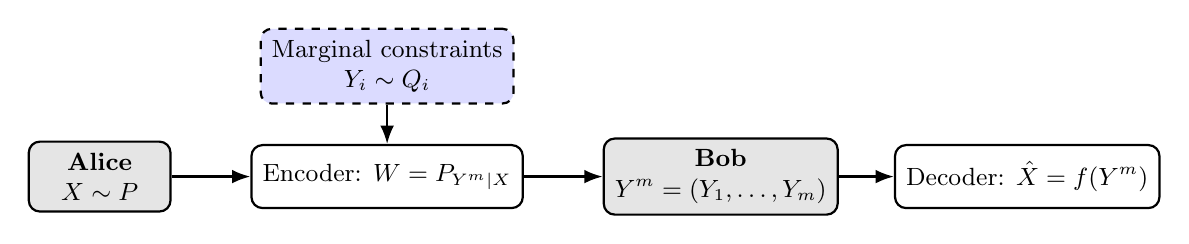
\begin{tikzpicture}[
    >=Latex,
    font=\small,
    node distance=1.2cm and 1.4cm,
    box/.style={draw, rounded corners, thick, align=center, minimum height=8mm},
    smallbox/.style={draw, rounded corners, thick, fill=gray!60, align=center, minimum height=7mm},
    constraint/.style={draw, rounded corners, thick, dashed, fill=blue!14, align=center},
    arr/.style={->, thick},
    every node/.style={inner sep=4pt}
]

% Left: source
\node[box, minimum width=1.8cm,fill=gray!20] (x) {\textbf{Alice} \\ $X\sim P$};

% Middle: encoder
\node[box, minimum width=2.8cm, right=1cm of x] (enc)
{Encoder: \(W=P_{Y^m|X}\)};

% Right top: representation
\node[box, minimum width=2.8cm, right=1cm of enc,fill=gray!20] (y)
{\textbf{Bob} \\ \(Y^m=(Y_1,\dots,Y_m)\)};

% Right bottom: decoder
\node[box, minimum width=2.2cm, right=0.7cm of y] (dec)
{Decoder: \(\hat X=f(Y^m)\)};

% Constraint box
\node[constraint, minimum width=2.3cm, above=0.5cm of enc] (cons)
{Marginal constraints\\ \(Y_i\sim Q_i\)};

% arrows
\draw[arr] (x) -- (enc);
\draw[arr] (enc) -- (y);
\draw[arr] (y) -- (dec);
\draw[arr] (cons) -- (enc);

\end{tikzpicture}
\caption{Marginal-constrained representation learning. A stochastic encoder \(W=P_{Y^m|X}\) maps the source \(X\sim P\) to a representation \(Y^m=(Y_1,\dots,Y_m)\), subject to the coordinate-wise output constraints \(Y_i\sim Q_i\). The decoder outputs \(\hat X=f(Y^m)\). The objective is to design \(W\) so that the representation reveals as much information about \(X\) as possible while respecting the prescribed marginals.}
\label{fig:marginal-constrained-repr}
\end{figure}

\section{List Entropy Coupling vs.\ Deterministic Randomness Extraction }\label{app:randomness}
As mentioned in Section~\ref{sec:intro}, in the classical deterministic randomness extraction setting, one observes i.i.d.\ samples $Z^m\sim Q^{\otimes m}$ and seeks a deterministic function $f$ such that $f(Z^m)\sim \Unif([k])$. At finite blocklength, this is often impossible due to arithmetic constraints. For example, if $Q=(1/3,2/3)$ on $\{0,1\}$, then every event under $Q^{\otimes m}$ has probability of the form $a/3^m$, and hence no deterministic function of finitely many i.i.d.\ samples can produce an exactly uniform bit. However, as mentioned earlier, there exists a coupling with marginals $Q$ such that $\Pr(Y_1\neq Y_2)=1/2$, yielding an exactly uniform bit via $X=\mathbf{1}\{Y_1\neq Y_2\}$.  One such coupling is the following: 
$$P_{Y_1,Y_2} = \begin{pmatrix}
   \tfrac1{12} & \tfrac1{4}\\
    \tfrac1{4} & \tfrac5{12}
\end{pmatrix}.$$
Thus, exact extraction becomes possible in finitely many samples.


As another example, consider distributions $Q=(1/2,1/2)$ on $\{0,1\}$ and 
\(P=\Unif([3])=(1/3,1/3,1/3)\) on $\{1,2,3\}$.
Then no deterministic function of \(m\) i.i.d.\ samples from \(Q\) can have distribution \(P\) for any finite \(m\), since under \(Q^{\otimes m}\) every event has probability of the form \(a/2^m\), whereas \(1/3\) is never of this form. Thus classical i.i.d.\ deterministic exact extraction/simulation is impossible.

In contrast, our coupling-based model allows this exactly with \(m=2\). Indeed, let \((Y_1,Y_2)\) be a coupling with marginals \(Q\) and joint distribution
\[
\begin{pmatrix}
\tfrac13 & \tfrac16\\
\tfrac16 & \tfrac13
\end{pmatrix},
\]
where rows and columns correspond to \(0,1\). Then \(Y_1\sim Q\) and \(Y_2\sim Q\), but the coordinates are dependent. Now define
\[
X=
\begin{cases}
1, & (Y_1,Y_2)=(0,0),\\
2, & (Y_1,Y_2)\in\{(0,1),(1,0)\},\\
3, & (Y_1,Y_2)=(1,1).
\end{cases}
\]
We then have
\[
\Pr(X=1)=1/3,\qquad
\Pr(X=2)=1/6+1/6=1/3,\qquad
\Pr(X=3)=1/3,
\]
so \(X\sim \Unif([3])\). Hence
\[H_2(\Unif([3])\|Q)=0.\]
This shows that even when the target alphabet differs from the source alphabet, the real gain in our framework comes from allowing dependence among the representation coordinates: such dependence can remove finite-block exact-simulation obstructions that are unavoidable under i.i.d.\ sampling. 

More generally, we can say that under classical i.i.d.\ setting, extraction from $m$ samples of $\Unif([k])$ to $\Unif([r])$ is possible if and only if $r| k^m$. Our framework removes this arithmetic constraint: by designing dependence among the coordinates while preserving the marginals, perfect extraction can be achieved even when $r \nmid k^m$. 

We remark that Corollary~\ref{cor:extraction} is straightforward from Theorem~\ref{thm:equalZero} and thus its proof is omitted. 


\section{Proof of Proposition~\ref{Prop:Binary_m}}\label{app:examples}
Before we give the proof, we provide an intuition behind the proof. 
Suppose $p,q\le \tfrac12$. The variables $Y_1,\dots,Y_m\sim \Ber(q)$ can collectively allocate at most $mq$ mass to the event $\{Y^m\neq 0\}$, since $\mathbf{1}\{Y^m\neq 0\}\le \sum_{i=1}^m Y_i$ and thus  the nonzero configurations of $Y^m$ provide at most $mq$ total mass on
which $X=1$ can be encoded deterministically away from the all-zero atom. To
recover $X\sim\Ber(p)$ exactly, the coupling must allocate total mass $p$ to
the event $\{X=1\}$. If $p\le mq$, this mass can be placed entirely inside
$\{Y^m\neq \mathbf 0\}$, yielding $H_m(\Ber(p)\|\Ber(q))=0$. If $p>mq$, the nonzero region has insufficient capacity. 
%The excess mass $p-mq$ must be placed on the atom $Y^m=\mathbf 0$, where $X$ remains random.
%The optimal coupling therefore concentrates all residual uncertainty on this single atom and makes $X$ deterministic everywhere else. 
After assigning $X=1$ deterministically on the set $\{Y^m \neq \mathbf{0}\}$ of total mass $mq$, the remaining probability $p-mq$ is placed on the atom $Y^m=\mathbf{0}$, which has mass $1-mq$. Therefore, the conditional probability $\Pr(X=1|Y^m=\mathbf{0})$ is exactly $\frac{p-mq}{1-mq}$.

\begin{proof}[Proof of Proposition~\ref{Prop:Binary_m}]
We first give the proof for $m\geq 2$ and then for $m=1$. 
Notice that  
\[H_m(\Ber(p)\|\Ber(q)) =H_m(\Ber(1-p)\|\Ber(q)),\]
which is obtained by replacing $X$ with $1-X$, and
\[H_m(\Ber(p)\|\Ber(q))=H_m(\Ber(p)\|\Ber(1-q)),\]
obtained by replacing each $Y_i$ with $1-Y_i$. Hence it suffices to prove theorem for \(0\le p\le \tfrac12,\) and \(0\le q\le \tfrac12.\)



\noindent\underline{$\bf m\geq 2$:}
Under these assumptions, $r=p$ and $s=q$, so we must show
\[H_m(\Ber(p)\|\Ber(q))=\begin{cases}
0, & p\le mq,\\[1ex]
(1-mq)\,h_{\mathsf{b}}\!\left(\dfrac{p-mq}{1-mq}\right), & p>mq,
\end{cases}\]
To prove this result, we need to prove achievability and converse. We break down the achievability in three cases: (1) $0\le p\le q$, (2) $q\leq  p\le mq$, and (3) $p> mq$.

\paragraph{Case 1: Achievability when $0\le p\le q$.}
We construct $Y^m=(Y_1,\dots,Y_m)$ with the correct marginals and make $X$ a deterministic function of $Y^m$.

Let $\mathbf 1=(1,\dots,1)$ and let $\mathcal W_{m-1}$ denote the set of all binary vectors of length $m$ having exactly $m-1$ ones. Define a probability distribution on $\{0,1\}^m$ by
\[\Pr(Y^m=\mathbf 1)=p,\qquad \Pr(Y^m=\mathbf 0)=1-p-\frac{m(q-p)}{m-1},\]
and for $y\in\mathcal W_{m-1}$
\[\Pr(Y^m=y)=\frac{m(q-p)}{m-1}\cdot \frac1m,\]
and zero elsewhere.
Since $0\le p\le q\le \frac12$ and $m\ge 2$, all masses are nonnegative, indeed
\[1-p-\frac{m(q-p)}{m-1}=1-\frac{mq-p}{m-1} \ge 1-\frac{m/2}{m-1}\ge 0.\]
For each coordinate $j$, we have \(\Pr(Y_j=1)=p+\frac{m-1}{m}\cdot \frac{m(q-p)}{m-1}=q.\) Thus each $Y_j\sim \Ber(q)$.
Now define
\[X:=\mathbf 1\{Y^m=\mathbf 1\}.\]
Then $X$ is a deterministic function of $Y^m$, so \(H(X| Y^m)=0,\)
and \(\Pr(X=1)=\Pr(Y^m=\mathbf 1)=p.\)
Hence $X\sim\Ber(p)$ and
\[H_m(\Ber(p)\|\Ber(q))=0\qquad\text{for }0\le p\le q.\]

\paragraph{Case 2: Achievability when $q\le p\le mq$.}
Let
\[\beta:=\frac{mq-p}{m-1}\in[0,q].\]
Define a distribution on $\{0,1\}^m$ by
\[\Pr(Y^m=\mathbf 1)=\beta,\qquad \Pr(Y^m=\mathbf 0)=1-mq+(m-1)\beta=1-p,\]
\[\Pr(Y^m=e_i)=q-\beta,\qquad i=1,\dots,m,\]
and zero elsewhere, where $e_i$ is the vector with a single $1$ in position $i$.
All masses are nonnegative, and for each coordinate $j$, we have \(\Pr(Y_j=1)=\beta+(q-\beta)=q.\) Thus each $Y_j\sim\Ber(q)$.

Now define
\[X:=\mathbf 1\{Y^m\neq \mathbf 0\}.\]
Then $X$ is a deterministic function of $Y^m$, so \(H(X| Y^m)=0,\)
and \(\Pr(X=1)=\beta+m(q-\beta)=mq-(m-1)\beta=p.\) Hence $X\sim\Ber(p)$ and
\[H_m(\Ber(p)\|\Ber(q))=0
\qquad\text{for }q\le p\le mq.\]

\paragraph{Case 3: achievability when $p>mq$.}
Assume now $p>mq$. Since $p\le \frac12$, this implies $mq<\frac12$.

Define a distribution on $\{0, 1\}^m$ by  \[\Pr(Y^m=\mathbf 0)=1-mq,\qquad \Pr(Y^m=e_i)=q,\qquad i=1,\dots,m,\]
and no mass elsewhere. Then each coordinate marginal is Bernoulli$(q)$.
Given $Y^m$, define $X$ as follows: \(X=1\) deterministically on each \(e_i\) and on the atom $\mathbf 0$ set \(\Pr(X=1| Y^m=\mathbf 0)=\theta,\)
where $\theta\coloneqq \frac{p-mq}{1-mq}.$ Then
\[\Pr(X=1)=mq+(1-mq)\theta=p,\]
so $X\sim\Ber(p)$. Since the only nondeterministic atom is $\mathbf 0$ and 
\[H(X| Y^m)=(1-mq)\,h_{\mathsf{b}}(\theta)=(1-mq)\,h_{\mathsf{b}}\!\left(\frac{p-mq}{1-mq}\right).\]
Therefore
\[H_m(\Ber(p)\|\Ber(q))\le(1-mq)\,h_{\mathsf{b}}\!\left(\frac{p-mq}{1-mq}\right).\]

\paragraph{Converse when $p>mq$.}
Let $(X,Y^m)$ be any coupling with \(X\sim\Ber(p),\) and  \(Y_1,\dots,Y_m\sim\Ber(q).\)
Let
\[t_0:=\Pr(Y^m=\mathbf 0),\qquad x_0:=\Pr(X=1,Y^m=\mathbf 0).\]
Also let \(N:=Y_1+\cdots+Y_m.\)
Then $\mathbb E[N]=mq.$ Since $N\ge \mathbf 1_{\{N>0\}}$, we have  \(\Pr(N>0)\le \mathbb E[N]=mq,\) and hence
\[t_0=\Pr(N=0)\ge 1-mq.\]
Moreover,
\[p=x_0+\Pr(X=1,N>0)\le x_0+\Pr(N>0)\le x_0+mq,\]
implying \(x_0\ge p-mq.\) Now, we can write 
\[H(X| Y^m)=\sum_{y\in\{0,1\}^m}\Pr(Y^m=y)\,
h_{\mathsf{b}}\!\bigl(\Pr(X=1| Y^m=y)\bigr)\ge t_0\,h_{\mathsf{b}}\!\left(\frac{x_0}{t_0}\right).\]
Set \(T:=1-mq\) and \(\delta:=p-mq.\)
Then $t_0\ge T$ and $x_0\ge \delta$. Also, since $p\le \frac12$ and $mq<\frac12$,
\[T> \frac12,\qquad x_0\le p\le \frac12<T.\]
For fixed $x\in[0,\frac12]$, the map \(t\mapsto t\,h_{\mathsf{b}}(x/t)\)
is increasing on $[x,\infty)$, since
\[\frac{\partial}{\partial t}\Bigl[t\,h_{\mathsf{b}}(x/t)\Bigr]=\log\!\frac{t}{t-x}\ge 0,\]
implying 
\[t_0\,h_{\mathsf{b}}\!\left(\frac{x_0}{t_0}\right)\ge
T\,h_{\mathsf{b}}\!\left(\frac{x_0}{T}\right).\]
Now consider
\[f(x):=T\,h_{\mathsf{b}}(x/T),\]
for $x\in[0,T]$. This function is symmetric about $T/2$ and strictly increasing on $[0,T/2]$. Since \(\delta=p-mq\) and \(T-\delta=1-p\ge p,\) every $x\in[\delta,p]$ satisfies \[\min\{x,T-x\}\ge \delta.\]
Also, note that by symmetry and monotonicity, we have
\(f(x)\ge f(\delta),\) for $x\in[\delta,p]$. In particular,
\[T\,h_{\mathsf{b}}\!\left(\frac{x_0}{T}\right)\ge T\,h_{\mathsf{b}}\!\left(\frac{\delta}{T}\right)=(1-mq)\,h_{\mathsf{b}}\!\left(\frac{p-mq}{1-mq}\right).\]
Putting altogether, we can write
\[H(X| Y^m)\ge(1-mq)\,h_{\mathsf{b}}\!\left(\frac{p-mq}{1-mq}\right),\]
which is the desired converse result. 

Now, we prove the theorem for $m=1$.

\noindent\underline{$\bf m= 1$:} 
As before, it suffices to prove the result for \(0\le p\le \tfrac12,\) and \(0\le q\le \tfrac12.\) 

% \textbf{Step 1: Symmetries.}
% We first show that
% \[
% H_1(\Ber(p)\|\Ber(q))
% =
% H(\Ber(1-p)\|\Ber(q))
% =
% H(\Ber(p)\|\Ber(1-q)).
% \]
% Indeed, if $(X,Y)$ is any coupling with $X\sim \Ber(p)$ and $Y\sim \Ber(q)$, then
% \[
% (1-X,Y)
% \]
% is a coupling of $\Ber(1-p)$ and $\Ber(q)$, and since the map $x\mapsto 1-x$ is bijective,
% \[
% H(1-X| Y)=H(X| Y).
% \]
% Taking the infimum over all couplings gives
% \[
% H(\Ber(1-p)\|\Ber(q))
% \le
% H_1(\Ber(p)\|\Ber(q)).
% \]
% Applying the same argument with $p$ replaced by $1-p$ yields the reverse inequality, hence equality. The proof of
% \[
% H_1(\Ber(p)\|\Ber(q))
% =
% H(\Ber(p)\|\Ber(1-q))
% \]
% is identical, replacing $Y$ by $1-Y$.

% Therefore
% \[
% H_1(\Ber(p)\|\Ber(q))
% =
% H(\Ber(r)\|\Ber(s)),
% \]
% where
% \[
% r=\min\{p,1-p\},
% \qquad
% s=\min\{q,1-q\}.
% \]
% Since $r,s\in[0,\frac12]$, it suffices to compute
% \[
% H_1(\Ber(p)\|\Ber(q))
% \qquad\text{under the assumption}\qquad
% 0\le p\le \frac12,\ \ 0\le q\le \frac12.
% \]

Fix $p,q\in[0,\frac12]$. Let $(X,Y)$ be any coupling with
\(X\sim \Ber(p)\) and \(Y\sim \Ber(q).\) Define
\[a:=\Pr(X=1| Y=0),
\qquad b:=\Pr(X=1| Y=1).\]
Then $a,b\in[0,1]$, and since $\Pr(Y=1)=q$ and $\Pr(Y=0)=1-q$, we must have \(\Pr(Y=1)=(1-q)a+qb.\) Similarly, since $X\sim \Ber(p)$, we must have \((1-q)a+qb=p.\)
Conversely, for any $a,b\in[0,1]$ satisfying
\((1-q)a+qb=p,\) if we let $Y\sim \Ber(q)$ and define the conditional law of $X$ by
\[\Pr(X=1| Y=0)=a,\qquad \Pr(X=1| Y=1)=b,\] then $X\sim \Ber(p)$.
Thus the optimization problem is exactly
\[H_1(\Ber(p)\|\Ber(q))
= \min\Bigl\{(1-q)h_{\mathsf{b}}(a)+q\,h_{\mathsf{b}}(b):\ 0\le a,b\le 1,\ (1-q)a+qb=p\Bigr\}.\]
Set
\[F(a,b):=(1-q)h_{\mathsf{b}}(a)+q\,h_{\mathsf{b}}(b).\]
Since $h_{\mathsf{b}}$ is concave on $[0,1]$, $F$ is concave on $[0,1]^2$. The feasible set
\[\mathcal S:=\{(a,b)\in[0,1]^2:(1-q)a+qb=p\}\]
is a compact line segment. A concave function on a compact line segment attains its minimum at an endpoint of the segment. Hence it remains to determine the endpoints of $\mathcal S$ and compare the corresponding values of $F$.

Now we consider two cases. 
\paragraph{Case 1: $p\le q$.}
The line \((1-q)a+qb=p\) meets the sides $a=0$ and $b=0$ of the unit square at
\[(0,p/q) \qquad\text{and}\qquad\Big(\frac{p}{1-q},0\Big),\]
respectively. Since $p\le q$ and $p\le 1-q$, both points lie in $[0,1]^2$. These are the two endpoints of $\mathcal S$. Therefore
\[H_1(\Ber(p)\|\Ber(q))
=\min\left\{
q\,h_{\mathsf{b}}\!\left(\frac{p}{q}\right),
\,(1-q)\,h_{\mathsf{b}}\!\left(\frac{p}{1-q}\right)
\right\}.\]
We now show that the first term is the smaller one. Fix $p\in[0,\frac12]$ and define \(\phi(t):=t\,h_{\mathsf{b}}(p/t)\) for $t\ge p$.
A direct differentiation gives
\[\phi'(t)=\log_2\!\frac{t}{t-p}\ge 0,\]
so $\phi$ is increasing on $[p,\infty)$. Since $q\le 1-q$, we have 
\[q\,h_{\mathsf{b}}\!\left(\frac{p}{q}\right) =\phi(q)\le\phi(1-q)=(1-q)\,h_{\mathsf{b}}\!\left(\frac{p}{1-q}\right).\]
Hence
\[H_1(\Ber(p)\|\Ber(q))=q\,h_{\mathsf{b}}\!\left(\frac{p}{q}\right)
\qquad\text{when } p\le q.\]

\paragraph{Case 2: $p>q$.}
Again, since $p\le \frac12\le 1-q$, the line \((1-q)a+qb=p\)
meets the sides $b=0$ and $b=1$ at \[
\Big(\frac{p}{1-q},0\Big) \qquad\text{and}\qquad \Big(\frac{p-q}{1-q},1\Big),\]
and these are the two endpoints of $\mathcal S$. Therefore
\[H_1(\Ber(p)\|\Ber(q))=\min\left\{
(1-q)\,h_{\mathsf{b}}\!\left(\frac{p}{1-q}\right),\,(1-q)\,h_{\mathsf{b}}\!\left(\frac{p-q}{1-q}\right)\right\}.\]
Using the symmetry $h_{\mathsf{b}}(u)=h_{\mathsf{b}}(1-u)$, the first term can be rewritten as
\[
(1-q)\,h_{\mathsf{b}}\!\left(\frac{1-p-q}{1-q}\right).
\]
Now
\[
0\le \frac{p-q}{1-q}\le \frac{1-p-q}{1-q}\le \frac12,
\]
because $q\le p\le \frac12$. Since $h_{\mathsf{b}}$ is increasing on $[0,\frac12]$, it follows that
\[
h_{\mathsf{b}}\!\left(\frac{p-q}{1-q}\right)
\le
h_{\mathsf{b}}\!\left(\frac{1-p-q}{1-q}\right)
=
h_{\mathsf{b}}\!\left(\frac{p}{1-q}\right).
\]
Hence
\[
H_1(\Ber(p)\|\Ber(q))
=
(1-q)\,h_{\mathsf{b}}\!\left(\frac{p-q}{1-q}\right)
\qquad\text{when } p>q.
\]

Combining the two cases, for all $0\le p,q\le \frac12$,
\[
H_1(\Ber(p)\|\Ber(q))
=
\begin{cases}
q\,h_{\mathsf{b}}\!\left(\dfrac{p}{q}\right), & p\le q,\\[1.2ex]
(1-q)\,h_{\mathsf{b}}\!\left(\dfrac{p-q}{1-q}\right), & p>q.
\end{cases}
\]
\end{proof}

\section{Proofs of Results in Section~\ref{sec:main}}
% \begin{proof}[Proof of Theorem~\ref{thm:homogeneous-exp}]
% We use the quantile coupling (inverse CDF) method: 
% we generate both $X\sim P$ and $Y^m\coloneqq (Y_1, \dots, Y_m)\sim Q^{\otimes m}$ from a common uniform variable $U\sim \mathsf{Unif}[0,1)$ via their respective inverse-CDF (interval partition) representations. The partition for $X$ has only $r-1$ boundary points. Each realization of $Y^m$ corresponds to an interval $I_j$ of length at most $M^m$, where $M:=\|Q\|_\infty$. If $I_j$ does not contain any boundary point, then it lies entirely within a single $P$-interval, so $Y^m$ uniquely determines $X$. Hence, ambiguity arises only when $I_j$ intersects one of the $r-1$ boundaries, which occurs with probability at most $(r-1)M^m$.

% Write $\mathcal X=\{x_1,\dots,x_r\}.$ We construct a coupling of $X\sim P$ and $Y_i\sim Q$ for $i\in[m]$.  For each $a=(a_1,\dots,a_m)\in \mathcal X^m$, define
% \[
% q_m(a):=\prod_{i=1}^m Q(a_i).
% \]
% Choose an arbitrary ordering $\mathcal X^m=\{a^{(1)},\dots,a^{(N)}\},$ with $N=r^m$, and partition $[0,1)$ into half-open intervals
% \[
% I_j:=\Bigl[\sum_{k<j} q_m(a^{(k)}),\ \sum_{k\le j} q_m(a^{(k)})\Bigr),
% \]
% for $j\in[N]$. Then $|I_j|=q_m(a^{(j)}),$ and if $U\sim \mathsf{Unif}[0,1)$, the rule
% \[
% Y^m=(Y_1,\dots,Y_m)=a^{(j)}
% \quad\text{whenever }U\in I_j
% \]
% produces $Y^m\sim Q^{\otimes m}$, so that $Y_i\sim Q$.  

% Next, partition $[0,1)$ according to $P$:
% \[
% J_\ell:=\Bigl[\sum_{k<\ell} P(x_k),\ \sum_{k\le \ell} P(x_k)\Bigr),
% \]
% for $\ell\in[r]$.
% Then $\{J_\ell\}_{\ell=1}^r$ is a partition of $[0,1)$ and $|J_\ell|=P(x_\ell).$ Consider the rule
% \[
% X:=x_\ell
% \quad\text{whenever }U\in J_\ell.
% \]
% Then $X\sim P$. Thus $(X,Y_1,\dots,Y_m)$ is a valid coupling of $(P,Q,\dots,Q)$.

% Now let
% \[
% \mathcal B:=\Bigl\{\sum_{k\le \ell} P(x_k):\ \ell=1,\dots,r-1\Bigr\}
% \]
% be the set of interior boundary points of the partition $\{J_\ell\}_{\ell=1}^r$.
% Define the ambiguity event
% \[
% \mathcal A:=\Bigl\{U\in I_j\text{ for some }j\text{ such that }I_j\cap \mathcal B\neq\varnothing\Bigr\},
% \]
% and let $A$ be its indicator. 
% On the event $\{A=0\}$, the interval $I_j$ lies entirely inside a single interval $J_\ell$, so $Y^m$ uniquely determines $X$, and hence
% \[
% H(X| Y^m,A=0)=0.
% \]

% There are $(r-1)$ boundary points in $\mathcal B$, and each belongs to exactly one interval $I_j$. Hence
% \begin{align*}
%     \Pr(A=1) &\le (r-1)\max_{1\le j\le N}|I_j|\\
%     & = (r-1)\max_{a\in\mathcal X^m} q_m(a)\\
%     & \le (r-1)M^m \eqqcolon \zeta_m.
% \end{align*}

% Since $A$ is a function of $Y^m$, we have $H(X| Y^m)=H(X| Y^m,A)$, and therefore
% \begin{align*}
% H(X| Y^m)
% &=\Pr(A=1)\,H(X| Y^m,A=1)\\
% &\le \zeta_m \log r.
% \end{align*}
% Taking the infimum over all couplings yields
% \[
% H_m(P\|Q)\le \zeta_m\log r.
% \]
% \end{proof}

We begin by proving Theorem~\ref{thm:homogeneous-exp}. However, instead of proving this theorem, we prove the more general result for the heterogeneous case which was stated in Theorem~\ref{thm:heterogeneous-exp}. Assuming $Q_i = Q$ in this theorem, we recover Theorem~\ref{thm:homogeneous-exp}.

\begin{proof}[Proof of Theorem~\ref{thm:heterogeneous-exp}]
We use the quantile coupling (inverse CDF) method: 
We generate both $X\sim P$ and the list $Y^m\coloneqq (Y_1, \dots, Y_m)\sim Q_1\otimes \dots\otimes Q_m$ from a common uniform variable $U\sim \mathsf{Unif}[0,1)$ via their respective inverse-CDF (interval partition) representations. The partition for $X$ has only $r-1$ boundary points. Each realization of $Y^m$ corresponds to an interval $I_j$ of length at most $M^m$. If $I_j$ does not contain any boundary point, then it lies entirely within a single $P$-interval, so $Y^m$ uniquely determines $X$. Hence, ambiguity arises only when $I_j$ intersects one of the $r-1$ boundaries, which occurs with probability at most $(r-1)M^m$.

Write $\mathcal X=\{x_1,\dots,x_r\}.$ We construct a coupling of $X\sim P$ and $Y_i\sim Q_i$ for $i\in[m]$.  For each $a=(a_1,\dots,a_m)\in \mathcal X^m$, define
\[
q_m(a):=\bigotimes_{i=1}^m Q_i(a_i).
\]
Choose an arbitrary ordering $\mathcal X^m=\{a^{(1)},\dots,a^{(N)}\},$ with  $N=r^m$, and partition $[0,1)$ into half-open intervals
\[
I_j:=\Bigl[\sum_{k<j} q_m(a^{(k)}),\ \sum_{k\le j} q_m(a^{(k)})\Bigr),
\]
for $j\in[N]$. Then $|I_j|=q_m(a^{(j)}),$ and if $U\sim \mathsf{Unif}[0,1)$, the rule
\[
Y^m:=(Y_1,\dots,Y_m)=a^{(j)}
\quad\text{whenever }U\in I_j
\]
produces
\[
\Pr(Y^m=a)=q_m(a)=\bigotimes_{i=1}^m Q_i(a_i),
\]
so that $Y_i\sim Q_i$.  Next, partition $[0,1)$ according to $P$:
\[
J_\ell:=\Bigl[\sum_{k<\ell} P(x_k),\ \sum_{k\le \ell} P(x_k)\Bigr),
\]
for $\ell\in[r]$.
Then $\{J_\ell\}_{\ell=1}^r$ is a partition of $[0,1)$ and $|J_\ell|=P(x_\ell).$ Consider the rule $X:=x_\ell$ whenever  $U\in J_\ell$. 
Then $X\sim P$. Thus $(X,Y_1,\dots,Y_m)$ is a valid coupling of $(P,Q_1,\dots,Q_m)$.
Now let
\[
\mathcal B:=\Bigl\{\sum_{k\le \ell} P(x_k):\ \ell=1,\dots,r-1\Bigr\}
\]
be the set of interior boundary points of the partition $\{J_\ell\}_{\ell=1}^r$.
Define the ambiguity event
\[
\mathcal A:=\Bigl\{U\in I_j\text{ for some }j\text{ such that }I_j\cap \mathcal B\neq\varnothing\Bigr\},
\]
which is a function of $Y^m$. Define $A$ as the indicator of $\mathcal A$. 
On the event $\{A=0\}$, the interval $I_j$ containing $U$ lies entirely inside a
single interval $J_\ell$ for some $\ell$. Hence, once $Y^m=a^{(j)}$ is known, the value of $X$ is uniquely determined. Therefore
\(H(X| Y^m,A=0)=0.\)

We next bound $\Pr(A=1)$. There are exactly $(r-1)$ points in $\mathcal B$, and each such point belongs to exactly one interval $I_j$. Hence
\begin{align*}
    \Pr(A=1) &\le (r-1)\max_{1\le j\le N}|I_j|\\
    & = (r-1)\max_{a\in\mathcal X^m} q_m(a)\\
    & \leq \min\{1, (r-1) M^m\} \eqqcolon \zeta_m.
\end{align*}

Since $A$ is a function of $Y^m$, we have $H(A| Y^m)=0,$ and therefore $H(X| Y^m) = H(X| Y^m,A)$. Thus, we can write
\begin{align*}
H(X| Y^m) &=\Pr(A=1)\,H(X| Y^m,A=1) +\Pr(A=0)\,H(X| Y^m,A=0)\\
& = \Pr(A=1)\,H(X| Y^m,A=1)\\
& \leq  \zeta_m \, H(X| Y^m,A=1)\\
& \leq  \zeta_m \, \log r.
\end{align*}
Since $H(P\|Q_1,\dots,Q_m)$ is the infimum of $H(X| Y^m)$ over all couplings, we conclude that
\(H(P\|Q_1,\dots,Q_m)\le \zeta_m\log r.\)


\end{proof}

\begin{proof}[Proof of Theorem~\ref{thm:equalZero}]
We first prove the result under the stronger assumption $\ell=1$, i.e., $Q(x)>0$ for all $x\in[r]$, and then extend to general $\ell$.

Fix $n\ge 1$, and write $\mu_n:=Q^{*n}$ for the $n$-fold convolution of $Q$ on $[r]$ and $q_{\min}$ for the $\min_{x\in [r]} Q(x)$. Since $Q(x)\ge q_{\min}$ for every $x$, the transition kernel
\[
K(x,y):=Q(y-x), \qquad x,y\in[r],
\]
satisfies the minorization
\[
K(x,\cdot)\ge rq_{\min}\,U_r(\cdot),
\qquad\forall x\in[r],
\]
where $U_r$ is the law of $\mathsf{Uniform}([r])$.
Since $U_r$ is an invariant measure for $K$, the Doeblin contraction bound gives
\[
\TV(\mu_n,U_r)\le (1-rq_{\min})^n.
\]

Since $U_r$ is shift-invariant, it follows that for every $j\in[r]$,
\begin{equation}\label{eq:couplingproof1}
  \TV(\mu_n,\tau_{-j}\mu_n)
\le 2\,\TV(\mu_n,U_r)
\le 2(1-rq_{\min})^n,  
\end{equation}

where $\tau_{j}$ is the shift operator.

Now fix $j\in[r]$, and let $(A_j,B_j)$ be a maximal coupling of $\mu_n$ and $\tau_{-j}\mu_n$.
Define
\[
T_j:=B_j+j \pmod r
\qquad \text{and} \qquad
D_j:=T_j-A_j \pmod r.
\]
Then both $A_j$ and $T_j$ have law $\mu_n$, and on the event $\{A_j=B_j\}$ we have $D_j=j$.
Hence
\begin{align*}
\TV(\mathsf{Law}(D_j),\delta_j)
&= \Pr(D_j \neq j)\\
&\le \Pr(A_j\neq B_j)\\
&= \TV(\mu_n,\tau_{-j}\mu_n)\\
&\le 2(1-rq_{\min})^n.
\end{align*}

Let $M_n$ be the $r\times r$ matrix whose $j$th column is $\mathsf{Law}(D_j)$.
Thus we need to show that there exists $w\in \Delta([r])$ such that $M_n w = P$.
Since each column of $M_n$ is within total variation distance at most $2(1-rq_{\min})^n$ of the corresponding simplex vertex $\delta_j$, we have
\[
\|M_n-I\|_1 \le 4(1-rq_{\min})^n,
\]
where $\|\cdot\|_1$ is the operator norm induced by $\ell_1$ norm, i.e., the maximum column sum norm. Assume now that
\[
(1-rq_{\min})^n<\frac{p_{\min}}{8},
\]
with $p_{\min}>0$. Since $p_{\min}\le 1$, this implies $\|M_n-I\|_1<1/2$, so $M_n$ is invertible and
\[
\|M_n^{-1}\|_1\le \frac{1}{1-\|M_n-I\|_1}\le 2.
\]
Let \(w:=M_n^{-1}P.\) Then, we can write 
\begin{align*}
\|w-P\|_1 & = \|M_n^{-1}(I-M_n)P\|_1\\
& \le \|M_n^{-1}\|_1\,\|I-M_n\|_1\,\|P\|_1\\
& \le 8(1-rq_{\min})^n\\
& < p_{\min}.
\end{align*}
Therefore, for every $j\in[r]$,
\[
w(j)\ge P(j)-\|w-P\|_1 >0.
\]
Also, since every column of $M_n$ sums to $1$, we have \(w\in\Delta([r])\).
Thus
\[
P=\sum_{j\in[r]} w(j)\mathsf{Law}(D_j).
\]

We now realize each $D_j$ from a valid coupling of $2n$ copies of $Q$.
For each $s\in[r]$, let $\alpha_s$ be the conditional law of $(Z_1,\dots,Z_n)$ given that
\[
Z_1+\cdots+Z_n\equiv s \pmod r,
\]
where $Z_1,\dots,Z_n\stackrel{iid}{\sim} Q$.
This is well defined because $\mu_n(s)>0$ for all $s$.
Given $(A_j,T_j)=(s,t)$, sample $(Y_1,\dots,Y_n)\sim \alpha_s$ and $(Y_{n+1},\dots,Y_{2n})\sim \alpha_t$ independently.
Let $\pi^{(j)}$ be the resulting law on $([r])^{2n}$.
Although the conditional law \(\alpha_s\) does not itself have one-dimensional marginals \(Q\), the unconditional first block under \(\pi^{(j)}\) has law
\[
\sum_{s\in[r]} \Pr(A_j=s)\,\alpha_s
=
\sum_{s\in[r]} \mu_n(s)\,\alpha_s
=
Q^{\otimes n},
\]
by the law of total probability. Similarly, the unconditional second block has law
\[
\sum_{t\in[r]} \Pr(T_j=t)\,\alpha_t
=
\sum_{t\in[r]} \mu_n(t)\,\alpha_t
=
Q^{\otimes n},
\]
since \(T_j\sim \mu_n\). Therefore each coordinate under $\pi^{(j)}$ has marginal $Q$. 

Now define
\[
f(y_1,\dots,y_{2n})
:=
\Bigl(\sum_{i=n+1}^{2n} y_i\Bigr)-\Bigl(\sum_{i=1}^n y_i\Bigr)
\pmod r.
\]
Under $\pi^{(j)}$, the first block sum is $A_j$ and the second is $T_j$, so
\[
f_\#\pi^{(j)}=\mathsf{Law}(D_j).
\]

Finally, let
\[
\pi:=\sum_{j\in[r]} w(j)\pi^{(j)}.
\]
Then every one-dimensional marginal of $\pi$ is $Q$, and
\[
f_\#\pi=P.
\]
Therefore, if $(Y_1,\dots,Y_{2n})\sim \pi$ and we set \(X:=f(Y_1,\dots,Y_{2n}),\)
then $H(X| Y_1,\dots,Y_{2n})=0$.
Hence \(H_{2n}(P\|Q)=0.\)

If $m\ge 2n$, we may append extra coordinates with marginal $Q$ arbitrarily. Then $X$ remains a deterministic function of the full list, so $H_m(P\|Q)=0$ as well.
Thus any $n_0$ satisfying
\[
(1-rq_{\min})^{n_0}<\frac{p_{\min}}{8}
\]
yields the conclusion with $m_0=2n_0$. Thus, one may choose $m_0$ to be 
\[m_0=2\left\lceil
\frac{\log(8/p_{\min})}{-\log(1-rq_{\min})}
\right\rceil. %= \Theta\big(\log1/p_{\min}\big).
\]

It remains to show the result for general $\ell > 1$. If $Q$ does not have full support, let $\ell$ be such that $Q^{*\ell}$ has full support.
Group the variables into blocks of length $\ell$:
\[
W_t := Y_{(t-1)\ell+1}+\cdots+Y_{t\ell}\pmod r.
\]
Then each $W_t$ has distribution $Q^{*\ell}$.
Applying the above construction to $(W_1,\dots,W_{2n})$ yields exact recovery using $2n$ blocks, i.e., $2n\ell$ original samples.
This proves the claim with
\[
m_0 = 2\ell n_0
=
2\ell \left\lceil
\frac{\log(8/p_{\min})}{-\log(1-r\widetilde q_{\min})}
\right\rceil.
\]
\end{proof}

% %%%%%%%%%%%%%%%%%%%%%%%%%%%%%%%%%%%%%%%%%%%%%%%%%%%%%%%%%%%%

\begin{proof}[Proof of Corollary~\ref{cor:equalZero-arbitrary-support}]
Let \(S:=\supp(P)\), \(s:=|S|\), and \(t:=r-s\). Fix any \(x_0\in S\) and define
\(\zeta:=\frac{p_{\min}}{2(t+1)}\). Construct \(\widetilde P\in\Delta([r])\) by
\[
\widetilde P(x)=
\begin{cases}
\zeta, & x\notin S,\\
P(x), & x\in S\setminus\{x_0\},\\
P(x_0)-t\zeta, & x=x_0.
\end{cases}
\]
Then \(\widetilde P\) is a valid distribution with full support: the total mass is preserved, and since \(t\zeta< p_{\min}\le P(x_0)\), we have \(\widetilde P(x_0)>0\), while all other entries are clearly positive. Moreover, \(\widetilde p_{\min}:=\min_x \widetilde P(x)\ge \zeta=\frac{p_{\min}}{2(r-s+1)}\).

Now define the deterministic map \(g:[r]\to[r]\) by
\[g(x)=\begin{cases}
x, & x\in S,\\
x_0, & x\notin S.
\end{cases}\]
We can now show that \(g_{\#}\widetilde P=P\). Indeed, if \(x\in S\setminus\{x_0\}\), then \(g^{-1}(\{x\})=\{x\}\), so
\(g_{\#}\widetilde P(x)=\widetilde P(x)=P(x).\)
For \(x=x_0\), we have \(g^{-1}(\{x_0\})=\{x_0\}\cup([r]\setminus S),\)
hence
\[g_{\#}\widetilde P(x_0)=\widetilde P(x_0)+\sum_{x\notin S}\widetilde P(x)=\bigl(P(x_0)-t\zeta\bigr)+t\zeta
=P(x_0).\]
Finally, if \(x\notin S\), then \(g_{\#}\widetilde P(x)=0=P(x)\). Thus $g_{\#}\widetilde P=P.$

Applying Theorem~\ref{thm:equalZero} to $\widetilde P$ gives \(H_m(\widetilde P\|Q)=0\) for all
\[
m \ge 2\ell\left\lceil \frac{\log(8/\widetilde p_{\min})}{-\log(1-r\widetilde q_{\min})} \right\rceil.
\]
Using \(\widetilde p_{\min}\ge p_{\min}/(2(r-s+1))\), it suffices to take
\[
m \ge 2\ell\left\lceil \frac{\log\bigl(16(r-s+1)/p_{\min}\bigr)}{-\log(1-r\widetilde q_{\min})} \right\rceil.
\]

For every such \(m\), there exists a coupling \((\widetilde X,Y_1,\dots,Y_m)\) with \(\widetilde X\sim \widetilde P\), \(Y_i\sim Q\), and \(\widetilde X=f(Y^m)\) a.s. Define \(X:=g(\widetilde X)=g(f(Y^m))\). Then \(X\sim P\), each \(Y_i\sim Q\), and \(X\) is a deterministic function of \(Y^m\). Hence \(H(X| Y^m)=0\), proving \(H_m(P\|Q)=0\).
\end{proof}

% \begin{proof}[Proof of Proposition~\ref{prop:dependent-exp}]
% We follow the construction in the proof of Theorem~\ref{thm:equalZero}. For simplicity, first consider the case $\ell=1$, and then extend by grouping samples into blocks.

% Fix $n\ge 1$, and let $\mu_n=Q^{*n}$. By the same argument as in Theorem~\ref{thm:equalZero}, we can construct a coupling of $(Y_1,\dots,Y_{2n})$ with $Y_i\sim Q$ and a deterministic function
% \[
% f(Y_1,\dots,Y_{2n})
% =
% \Bigl(\sum_{i=n+1}^{2n}Y_i-\sum_{i=1}^n Y_i\Bigr)\!\!\pmod r,
% \]
% such that the induced variable $X=f(Y_1,\dots,Y_{2n})$ satisfies the following property.

% There exists an event $A$, measurable with respect to $Y^m$, such that:
% (i) on $A^c$, $X$ is uniquely determined by $Y^m$, hence $H(X| Y^m,A=0)=0$, and
% (ii) $\mathbb{P}(A)\le \delta_n$, where $\delta_n\le 2(1-rq_{\min})^n$.

% Since $A$ is a function of $Y^m$, we have $H(A| Y^m)=0$, and therefore
% \[
% H(X| Y^m)
% =
% H(X| Y^m,A)
% =
% \mathbb{P}(A)\,H(X| Y^m,A=1).
% \]
% Using $H(X| Y^m,A=1)\le \log r$ and the standard decomposition
% \[
% H(X| Y^m)\le h_{\mathsf b}(\mathbb{P}(A)) + \mathbb{P}(A)\log r,
% \]
% we obtain
% \[
% H(X| Y^m)\le h_{\mathsf b}(\delta_n)+\delta_n\log r.
% \]

% For general $\ell\ge 1$, apply the same construction to block variables $W_t=\sum_{i=(t-1)\ell+1}^{t\ell}Y_i \pmod r$, whose common law is $Q^{*\ell}$ with full support. This yields the same bound with $\beta=1-r\widetilde q_{\min}$ and $m=2n\ell$.

% %The exponential rate follows from $\delta_n\le 2\beta^n$ and $m=2n\ell$.

% To prove the second part, choose \(n\) so that \(\delta_n\le \delta_\varepsilon\), where $\delta_\eps$ is the unique solution of  \[h_{\mathsf b}(\delta_\varepsilon)+\delta_\varepsilon\log r = \varepsilon.\] 
% Since the function \(\delta\mapsto h_{\mathsf b}(\delta)+\delta\log r\) is increasing on \([0,1/2]\), this implies
% \[H_{2n\ell}(P\|Q)\le h_{\mathsf b}(\delta_\varepsilon)+\delta_\varepsilon\log r\le \varepsilon.\]
% Hence \(m_\varepsilon(P\|Q)\le 2n\ell\). It therefore remains to ensure \(\delta_n\le \delta_\varepsilon\). Since \(\delta_n\le 2\beta^n\), it is enough to require \(2\beta^n\le \delta_\varepsilon,\)
% that is,
% \[n\ge \frac{\log(2/\delta_\varepsilon)}{-\log\beta}.\]
% Thus, we have 
% \[m_\varepsilon(P\|Q)\le2\ell\left\lceil \frac{\log(2/\delta_\varepsilon)}{-\log \beta}\right\rceil.\]
% Finally, it can be verified that $\delta_\eps\gtrsim \frac{\eps}{\log1/\eps} $, implying the desired result. 
% \end{proof}

\begin{proof}[Proof of Proposition~\ref{prop:dependent-exp}]
We first prove the claim for $\ell=1$. Write
\[
\mu_n:=Q^{*n},
\qquad
q_{\min}:=\min_{x\in[r]}Q(x),
\qquad
\beta:=1-rq_{\min}.
\]
As in the proof of Theorem~\ref{thm:equalZero} (specifically equation \eqref{eq:couplingproof1}), for each $j\in[r]$ there is a
coupling $\pi^{(j)}$ of $2n$ coordinates, each with marginal $Q$, such that
the decoder
\[
f(y_1,\ldots,y_{2n})
:=
\sum_{i=n+1}^{2n}y_i-\sum_{i=1}^n y_i
\pmod r
\]
satisfies
\[\Pr_{\pi^{(j)}}\bigl(f(Y^{2n})\neq j\bigr)\le2\beta^n .\]
Now draw $J\sim P$. Conditional on $J=j$, sample
$Y^{2n}\sim \pi^{(j)}$, and set $X:=J$. Then $X\sim P$, and since each
$\pi^{(j)}$ has one-dimensional marginals equal to $Q$, every coordinate
$Y_i$ also has marginal $Q$ under the mixture. Thus
$(X,Y_1,\ldots,Y_{2n})$ is a valid coupling.

Let $\widehat X:=f(Y^{2n})$. The decoder error satisfies
\[
\Pr(\widehat X\neq X)
=
\sum_{j\in[r]}P(j)\Pr_{\pi^{(j)}}(f(Y^{2n})\neq j)
\le
2\beta^n .
\]
Therefore, with
\(\delta_n:=\min\{1,2\beta^n\},\)
Fano's inequality gives
\[
H(X| Y^{2n})
\le
h_{\mathsf b}(\delta_n)+\delta_n\log r .
\]
Taking the infimum over all valid couplings yields the desired bound for
$\ell=1$.

For general $\ell$, apply the same argument to the block variables
\[
W_t:=\sum_{i=(t-1)\ell+1}^{t\ell}Y_i \pmod r,
\]
whose marginal law is $Q^{*\ell}$. Lifting each block-level coupling back to
$\ell$ original $Q$-coordinates by conditioning on the block sum preserves the
one-dimensional marginals. Replacing $q_{\min}$ by
\[
\widetilde q_{\min}:=\min_{x\in[r]}Q^{*\ell}(x)
\]
gives $\beta=1-r\widetilde q_{\min}$ and $m=2n\ell$, completing the proof.
\end{proof}







\section{Finite-Sample Exact Recovery Beyond Modular Sums}\label{app:ExactRecovery}
Theorems~\ref{thm:equalZero} and \ref{thm:equalZero-hetero} rely on modular block sums of independent $Q$-samples to achieve the finite-sample exact recovery. However, their proofs reveal that the modular-sum structure is not essential. What
matters is a block-level richness condition: after aggregating sufficiently
many $Q$-samples, the induced block distribution must be able to approximate
the simplex vertices well enough to span the target law. In this section, we formalize this generalization and provide examples of such richness conditions.   
\begin{theorem}\label{thm:hetero-unified}
Let $P\in\Delta([r])$ have full support, and let $Q_1,\dots,Q_m$ be distributions on arbitrary finite alphabets $\calY_1,\dots,\calY_m$. Fix an integer $\ell\ge1$ and assume, for simplicity, that $\ell$ divides $m$. For each block $t\in[m/\ell]$, let
$$
B_t=\{(t-1)\ell+1,\dots,t\ell\}.
$$
Suppose there exist deterministic maps
$$
\phi_t:\prod_{i\in B_t}\calY_i\to [r],
\qquad t\in [m/\ell],$$
such that, if $(Y_i)_{i\in B_t}\sim\bigotimes_{i\in B_t} Q_i$ and
$Z_t=\phi_t(\{Y_i\}_{i\in B_t}),$
then the law $R_t$ of $Z_t$ satisfies
$R_t(x)\ge \widetilde q_{\min}>0,$
for all $x\in[r]$ and for $t\in [m/\ell]$. Let
$$n_*:= \left\lceil \frac{\log(8/p_{\min})}{-\log(1-r\widetilde q_{\min})} \right\rceil,$$
with the convention that $n_*=1$ when $r\widetilde q_{\min}=1$. If $\frac{m}{\ell}\ge 2n_*,$ then $H(P\|Q_1,\dots,Q_m)=0.$ Equivalently, we have 
$$ m_0(P\|Q_1,\dots,Q_m) \le 2\ell \left\lceil \frac{\log(8/p_{\min})}{-\log(1-r\widetilde q_{\min})} \right\rceil.$$
\end{theorem}
\begin{proof}
Let $L=m/\ell$ and assume $L\ge 2n_*$. We use the first $2n_*$ blocks and append the remaining coordinates independently at the end.

For each block $t$, define
$$
Z_t=\phi_t((Y_i)_{i\in B_t}),
$$
where $(Y_i)_{i\in B_t}\sim\bigotimes_{i\in B_t}Q_i$, and let $R_t$ be the law of $Z_t$. By assumption,
$R_t(x)\ge \widetilde q_{\min}$ for all $x\in[r]$.
Set $\beta:=1-r\widetilde q_{\min}\in[0,1).$
We first show that sums of the $Z_t$'s are close to uniform. Since each $R_t$ dominates $\widetilde q_{\min}$ pointwise, we may write
$$R_t=r\widetilde q_{\min} U_r+\beta \overline R_t,$$
where $U_r$ is uniform on $[r]$ and $\overline R_t\in\Delta([r])$. Since convolution with $U_r$ gives $U_r$, it follows that for any collection of $n$ blocks,
$$
\TV(R_{t_1}*\cdots*R_{t_n},U_r)\le \beta^n.
$$
Let $\mu_1:=R_1*\cdots*R_{n_*}$ and  $\mu_2:=R_{n_*+1}*\cdots*R_{2n_*}.$
Then
$$
\TV(\mu_1,U_r)\le \beta^{n_*},
\qquad
\TV(\mu_2,U_r)\le \beta^{n_*}.
$$
For each $b\in[r]$, let $(A_b,B_b)$ be a maximal coupling of $\mu_1$ and $\tau_{-b}\mu_2$, where $\tau_{-b}$ denotes shift by $-b$ modulo $r$. Define
$$
T_b:=B_b+b \pmod r,
\qquad
D_b:=T_b-A_b \pmod r.
$$
Then $A_b\sim\mu_1$, $T_b\sim\mu_2$, and on the event $\{A_b=B_b\}$ we have $D_b=b$. Hence
$$
\TV(\mathsf{Law}(D_b),\delta_b)
\le
\Pr(A_b\ne B_b)
=
\TV(\mu_1,\tau_{-b}\mu_2)
\le
2\beta^{n_*}.
$$
Now let $M$ be the $r\times r$ matrix whose $b$th column is $\mathsf{Law}(D_b)$. Since the $b$th column is within total variation distance at most $2\beta^{n_*}$ of $\delta_b$, we have
$$
\|M-I\|_1\le 4\beta^{n_*}.
$$
By the choice of $n_*$, we have $\beta^{n_*}\leq \frac{p_{\min}}{8},$
unless $\beta=0$, in which case the same conclusion is immediate. Thus $\|M-I\|_1<1/2$, so $M$ is invertible by the Neumann series and
$\|M^{-1}\|_1\le 2.$
Let $w:=M^{-1}P$. Then
$$
\|w-P\|_1
=
\|M^{-1}(I-M)P\|_1
\le
\|M^{-1}\|_1\,\|I-M\|_1\,\|P\|_1
\le
8\beta^{n_*}
\leq 
p_{\min}.
$$
Thus $w(b)\ge P(b)-\|w-P\|_1\ge0$ for all $b$. Since the columns of $M$ sum to one, $w$ also sums to one, and hence $w\in\Delta([r])$. Consequently,
$$
P=\sum_{b\in[r]}w(b)\mathsf{Law}(D_b).
$$

It remains to realize this construction as a coupling of the original variables with the prescribed marginals. For each block $t$ and each $z\in[r]$, let $\alpha_{t,z}$ denote the conditional law of $(Y_i)_{i\in B_t}$ under $\bigotimes_{i\in B_t}Q_i$ given $\phi_t((Y_i)_{i\in B_t})=z$. This conditional law is well-defined because $R_t(z)\ge \widetilde q_{\min}>0$.

For the first group of $n_*$ blocks, let $\lambda_s^{(1)}$ be the conditional law of $(Z_1,\dots,Z_{n_*})$ given
$$
Z_1+\cdots+Z_{n_*}=s \pmod r
$$
under the product law $R_1\otimes\cdots\otimes R_{n_*}$. Define $\lambda_s^{(2)}$ analogously for $(Z_{n_*+1},\dots,Z_{2n_*})$.

Given $(A_b,T_b)=(s,t)$, sample
$$
(Z_1,\dots,Z_{n_*})\sim \lambda_s^{(1)},
\qquad
(Z_{n_*+1},\dots,Z_{2n_*})\sim \lambda_t^{(2)}.
$$
Then, conditional on each realized $Z_j=z$, sample the corresponding original block $(Y_i)_{i\in B_j}$ from $\alpha_{j,z}$, independently across blocks. This produces a coupling $\pi^{(b)}$ of the first $2n_*\ell$ coordinates.

Under $\pi^{(b)}$, each block has its original product marginal. Indeed, averaging over the block output gives
$$
\sum_{z\in[r]}R_j(z)\alpha_{j,z}
=
\bigotimes_{i\in B_j}Q_i.
$$
Thus every coordinate $Y_i$ has its prescribed marginal $Q_i$.
Now, define
$$f(Y_1,\dots,Y_{2n_*\ell})=\sum_{j=n_*+1}^{2n_*} Z_j-\sum_{j=1}^{n_*} Z_j\pmod r.$$
Under $\pi^{(b)}$, the law of $f$ is $\mathsf{Law}(D_b)$.

Finally, mix the couplings $\pi^{(b)}$ according to $w$:
$$
\pi_0:=\sum_{b\in[r]}w(b)\pi^{(b)}.
$$
Then every coordinate marginal remains correct and
$f_{\#}\pi_0=P.$
Thus, if $(Y_1,\dots,Y_{2n_*\ell})\sim\pi_0$ and $X=f(Y_1,\dots,Y_{2n_*\ell})$, then $X\sim P$ and
$H(X| Y_1,\dots,Y_{2n_*\ell})=0.$

If $m>2n_*\ell$, append the remaining coordinates $Y_{2n_*\ell+1},\dots,Y_m$ independently with their prescribed marginals $Q_{2n_*\ell+1},\dots,Q_m$. This preserves all marginal constraints, and since $X$ is already a deterministic function of the first $2n_*\ell$ coordinates, it remains a deterministic function of the full tuple. Therefore
$H(P\|Q_1,\dots,Q_m)=0.$
\end{proof}

The block-richness condition in Theorem~\ref{thm:hetero-unified} may look
abstract, but it can be verified under very primitive assumptions. The next
corollary shows that no common alphabet, convolution structure, or modular
operation is needed. It is enough that each marginal has two moderately likely
atoms. By grouping $\lceil\log_2 r\rceil$ such variables, we can manufacture an
$[r]$-valued block variable with full support.

\begin{corollary}[Two-heavy-atoms condition]\label{cor:two-heavy-atoms}
Let $P\in\Delta([r])$ have full support, and let $Q_1,\dots,Q_m$ be distributions on arbitrary finite alphabets. Assume that there exists $a>0$ such that each $Q_i$ has at least two atoms of mass at least $a$. Let
$$
k:=\lceil\log_2 r\rceil,
\qquad
q_0:=a^k.
$$
Assume, for simplicity, that $k$ divides $m$. If
$$
\frac{m}{k}
\ge
2\left\lceil
\frac{\log(8/p_{\min})}{-\log(1-rq_0)}
\right\rceil,
$$
then
$H(P\|Q_1,\dots,Q_m)=0.$
Equivalently,
\begin{equation}\label{eq:2heavySC_corollary}
m_0(P\|Q_1,\dots,Q_m)
\le
2\lceil\log_2 r\rceil
\left\lceil
\frac{\log(8/p_{\min})}
{-\log\!\bigl(1-r a^{\lceil\log_2 r\rceil}\bigr)}
\right\rceil.
\end{equation}
\end{corollary}
\begin{proof}
Let $k=\lceil\log_2 r\rceil$. Consider any block of $k$ coordinates. Since each $Q_i$ has at least two atoms of mass at least $a$, the product distribution over the block has at least $2^k\ge r$ atoms, each of probability at least $a^k$.

Choose $r$ such atoms and assign them injectively to the symbols in $[r]$. Assign all remaining atoms arbitrarily to symbols in $[r]$. This defines a deterministic map
$$
\phi_t:\prod_{i=(t-1)k+1}^{tk}\calY_i\to[r].
$$
Let $R_t$ be the law of the resulting block output. Since each symbol in $[r]$ receives at least one atom of mass at least $a^k$, we have $R_t(x)\ge a^k=q_0$ for all $x\in[r]$. The conclusion follows from Theorem~\ref{thm:hetero-unified} with $\ell=k$ and $\widetilde q_{\min}=q_0$.

Also note that since each $Q_i$ has two atoms of mass at least $a$, necessarily $a\le 1/2$.
As $r\le 2^k$, we have $rq_0=ra^k\le r2^{-k}\le 1$, so the denominator in equation~\eqref{eq:2heavySC_corollary} is well-defined, with the case $rq_0=1$ corresponding to the uniform block-output case.
\end{proof}

The intuition is simple. Each coordinate contributes a binary choice with
probability at least $a$ on each branch. A block of
$k=\lceil\log_2 r\rceil$ coordinates therefore contains at least $2^k\ge r$
product atoms, each with mass at least $a^k$. Assigning $r$ of these atoms to
the symbols in $[r]$ produces a block map whose pushforward has minimum mass at
least $q_0=a^k$. Theorem~\ref{thm:hetero-unified} then applies. Thus exact
recovery does not require algebraic structure; enough local randomness can be
grouped and binned into the block-level richness needed for the dependent
coupling.

Next, we show that the convolution structure presented in Theorems~\ref{thm:equalZero} and \ref{thm:equalZero-hetero} are special case of Theorem~\ref{thm:hetero-unified}. 

\begin{corollary}[Common block-convolution law]\label{cor:block-convolution-richness}
Let $P\in\Delta([r])$ have full support, and let $Q_1,\dots,Q_m\in\Delta([r])$. Fix $\ell\ge1$ and assume $\ell$ divides $m$. Suppose there exists a fully supported distribution $\widetilde Q\in\Delta([r])$ such that, for every $t=1,\dots,m/\ell$,
$$
Q_{(t-1)\ell+1}*\cdots*Q_{t\ell}=\widetilde Q.
$$
Let $\widetilde q_{\min}=\min_{x\in[r]}\widetilde Q(x)$. If
$$
\frac{m}{\ell}
\ge
2\left\lceil
\frac{\log(8/p_{\min})}{-\log(1-r\widetilde q_{\min})}
\right\rceil,
$$
then
$H(P\|Q_1,\dots,Q_m)=0.$
Equivalently,
$$
m_0(P\|Q_1,\dots,Q_m)
\le
2\ell
\left\lceil
\frac{\log(8/p_{\min})}{-\log(1-r\widetilde q_{\min})}
\right\rceil.
$$
\end{corollary}
\begin{proof}
Apply Theorem~\ref{thm:hetero-unified} with
$$
\phi_t(y_{(t-1)\ell+1},\dots,y_{t\ell})
=
\sum_{i=(t-1)\ell+1}^{t\ell} y_i
\pmod r.
$$
The law of $\phi_t$ under the product measure is precisely
$$
Q_{(t-1)\ell+1}*\cdots*Q_{t\ell}
=
\widetilde Q.
$$
Thus each block output law satisfies $R_t(x)\ge \widetilde q_{\min}$ for all $x\in[r]$, and the conclusion follows from Theorem~\ref{thm:hetero-unified}.
\end{proof}

\begin{remark}[Comparison of the two sufficient conditions]
Corollaries~\ref{cor:block-convolution-richness} and~\ref{cor:two-heavy-atoms} are two different ways of verifying the block-richness condition in Theorem~\ref{thm:hetero-unified}.

Corollary~\ref{cor:block-convolution-richness} is structurally sharper. It assumes that, after grouping the variables into blocks of length $\ell$, the modulo-$r$ block sums have a common fully supported law $\widetilde Q$. Under this alignment, the proof follows the same mechanism as Theorem~\ref{thm:equalZero}: block sums play the role of effective homogeneous observations. The resulting sample complexity is
$$
m_0
\lesssim
2\ell\,
\frac{\log(1/p_{\min})}{-\log(1-r\widetilde q_{\min})}.
$$
This bound can be small when the block convolution is well spread over $[r]$, but the assumption requires substantial structure across the heterogeneous marginals.

Corollary~\ref{cor:two-heavy-atoms} is more broadly applicable. It does not require the $Q_i$'s to live on the same alphabet, nor does it require any equality of block convolutions. It only requires that each marginal contain two atoms with probability at least $a$. The proof first converts each block of $k=\lceil\log_2 r\rceil$ heterogeneous samples into an $[r]$-valued variable by binning $r$ heavy product atoms. This yields the uniform lower bound $q_0=a^k$, and then Theorem~\ref{thm:hetero-unified} applies. The price for this generality is that the sample complexity becomes
$$
m_0
\lesssim
2\lceil\log_2 r\rceil\,
\frac{\log(1/p_{\min})}{-\log(1-r a^{\lceil\log_2 r\rceil})}.
$$

Thus, the two corollaries are not directly comparable. The block-convolution condition gives a sharper bound when the heterogeneous marginals have aligned aggregate structure. The two-heavy-atoms condition is less restrictive and works over arbitrary alphabets, but it may have worse constants because the guaranteed lower bound $a^{\lceil\log_2 r\rceil}$ can be small. Conceptually, the first corollary exploits existing convolutional richness, while the second manufactures such richness by grouping and binning.

In summary, the convolution-based construction exploits algebraic structure, whereas the two-heavy-atoms construction shows that such structure is not necessary—only minimal local randomness is required.
\end{remark}


Theorem~\ref{thm:hetero-unified} shows that the sum map is not essential; any block map whose pushforward has full support is enough. Thus, specialized to the homogeneous case, Theorem~\ref{thm:hetero-unified} implies the following. 
\begin{corollary}[Homogeneous block-map exact recovery]
Let $P\in\Delta([r])$ have full support and let $Q$ be a distribution on a finite alphabet $\calY$. Suppose there exist an integer $\ell\ge1$ and a deterministic map $\phi:\calY^\ell\to[r]$ such that, for
$$
Z=\phi(Y_1,\dots,Y_\ell),\qquad Y_1,\dots,Y_\ell\stackrel{iid}{\sim}Q,
$$
the law $R=\phi_\# Q^{\otimes \ell}$ satisfies
$$
\min_{x\in[r]}R(x)=q_\phi>0.
$$
Then $H_m(P\|Q)=0$ for all
$$
m\ge
2\ell
\left\lceil
\frac{\log(8/p_{\min})}{-\log(1-rq_\phi)}
\right\rceil.
$$
\end{corollary}
This corollary reduces to Theorem~\ref{thm:equalZero}  by taking $ \phi(y_1,\dots,y_\ell)=\sum_{i=1}^{\ell} y_i \pmod r,$ thus, $R=Q^{*\ell}$ and  
$q_\phi=\min_x Q^{*\ell}(x)=\widetilde q_{\min}.$ 
%While Theorem~\ref{thm:equalZero} uses the modulo-sum map to prove the finite-sample exact recovery,  Theorem~\ref{thm:hetero-unified} shows that the sum map is not essential; any block map whose pushforward has full support is enough.
Thus Theorem~\ref{thm:equalZero} is the modular-sum instance of a more general
principle: exact recovery only requires a block map whose pushforward has full
support.



\section{Finite-Sample Exact Recovery Under Different Coupling Structures}\label{app:coupling-structures}
\begin{figure}[t]
\centering
\includegraphics[scale=0.2]{coupling3.png}
\caption{
Hierarchy of coupling structures for finite-sample exact recovery. Independent and conditionally i.i.d.\ couplings are highly restricted. Conditionally independent couplings enable recovery by separating symbols across coordinates. General couplings are strictly more expressive: they shape the joint support of $(Y_1,\dots,Y_m)$ to enable exact recovery beyond coordinate-wise mechanisms.
}
\label{fig:coupling-hierarchy}
\end{figure}
In this section, we place the main result of Section~\ref{sec:main} into a broader perspective by isolating the precise role of \emph{dependence} in enabling finite-sample exact recovery. While Theorem~\ref{thm:equalZero} shows that general couplings can achieve $H_m(P\|Q)=0$ under mild conditions, it is far from obvious which structural features of the coupling make this possible.

To answer this, we compare four nested classes of couplings:
\begin{enumerate}
    \item Independent coupling: $Y_1,\dots,Y_m \sim Q$ i.i.d.\ and independent of $X$.
    \item Conditionally i.i.d.\ coupling: $Y_i | X=x \sim K_x$ i.i.d.\ across $i$ with kernels $\{K_x\}_{x\in \calX}$.
    \item Conditionally independent coupling: $Y_i | X=x \sim K_{i,x}$ independently across $i$, but not necessarily identically distributed with kernels $\{K_{i, x}\}_{i\in [m], x\in \calX}$.
    \item General coupling: arbitrary joint distribution with marginals $Y_i\sim Q$.
\end{enumerate}

These classes form a strict hierarchy, and, as we show, each step unlocks a fundamentally different mechanism for recovering $X$.

\begin{description}
    \item[Independent coupling:] If $Y^m\sim Q^{\otimes m}$ is independent of $X\sim P$, then $Y^m$ carries no information about $X$, and hence $H(X| Y^m)=H(P)$ for all $m$. In this regime, increasing $m$ only increases redundancy, not information.
    \item[Conditionally i.i.d.\ coupling:] Let $P,Q\in\Delta(\calX)$ and let $X\sim P$. Suppose that, conditional on $X=x$, the variables $Y_1,\dots,Y_m$ are i.i.d.\ with law $K_x$, and satisfy $\sum_{x\in\calX} P(x)K_x = Q.$
Then, it can be shown that  exact recovery is possible if and only if $H_1(P\|Q)=0$, implying that conditionally i.i.d.\ couplings do not enlarge the zero-entropy regime. 


\begin{proposition}
Let $P,Q\in\Delta(\calX)$ and let $X\sim P$. Suppose that, conditional on $X=x$, the variables $Y_1,\dots,Y_m$ are i.i.d.\ with law $K_x\in\Delta(\calX)$, and that the marginal constraint $\sum_{x\in\calX}P(x)K_x=Q$ holds. Then $H(X|Y^m)=0$ for some finite $m$ if and only if $H_1(P\|Q)=0$.
\end{proposition}

\begin{proof}
Let $S=\supp(P)$. Conditional on $X=x$, the law of $Y^m=(Y_1,\dots,Y_m)$ is $K_x^{\otimes m}$.

Suppose $H(X| Y^m)=0$. Then $X$ is a deterministic function of $Y^m$, and therefore the conditional laws $\{K_x^{\otimes m}:x\in S\}$ are mutually singular. Since $\calX$ is finite, $K_x^{\otimes m}$ and $K_{x'}^{\otimes m}$ are mutually singular if and only if $K_x$ and $K_{x'}$ are mutually singular. Indeed, if there exists $y\in\calX$ such that $K_x(y)>0$ and $K_{x'}(y)>0$, then $(y,\dots,y)$ has positive probability under both product measures, contradicting mutual singularity.

Thus the sets $A_x=\supp(K_x)$, $x\in S$, are pairwise disjoint. Since $Q=\sum_{x\in S}P(x)K_x$, we have $Q(A_x)=P(x)$ for every $x\in S$. Define $g:\calX\to\calX$ by $g(y)=x$ for $y\in A_x$, with arbitrary values outside $\cup_x A_x$. Then $g_\# Q=P$, so there exists a coupling of $X\sim P$ and $Y\sim Q$ such that $X=g(Y)$. Hence $H_1(P\|Q)=0$.

Conversely, if $H_1(P\|Q)=0$, then there exists a deterministic map $g$ such that $g_\#Q=P$. Let $K_x$ be the conditional law of $Y\sim Q$ given $g(Y)=x$. Then $\sum_xP(x)K_x=Q$, the supports of the $K_x$ are pairwise disjoint, and $X=g(Y_1)$ is already determined by the first coordinate. Therefore $H(X| Y^m)=0$.
\end{proof}
Conditionally i.i.d.\ couplings are repeated uses of the same observation
channel. Repetition may reduce uncertainty asymptotically, but it cannot
change the support geometry: if one observation cannot separate two values of
$X$, no finite number of identical observations can separate them exactly. Informally speaking $K_x^{\otimes m} \perp K_{x'}^{\otimes m}$ is equivalent to  $K_x \perp K_{x'}.$
Thus conditionally i.i.d.\ sampling creates no new finite-sample zero-entropy
regime.


\item[Conditionally independent coupling:] Allowing the conditional law to vary across coordinates fundamentally changes the picture. This is formalized in the following proposition. 
\begin{proposition}
Let $P\in\Delta(\calX)$ and suppose that, conditional on $X=x$, the variables $Y_1,\dots,Y_m$ are independent with laws $K_{i,x}$. Then $H(X| Y^m)=0$ if and only if for every $x\neq x'\in\supp(P)$ there exists $i\in[m]$ such that
$$
\supp(K_{i,x}) \cap \supp(K_{i,x'}) = \emptyset.
$$
\end{proposition}
\begin{proof}
Conditional on $X=x$, the law of $Y^m$ is $K_{1,x}\otimes\dots\otimes K_{m,x}$. Exact recovery holds if and only if these product measures are mutually singular over $x\in\supp(P)$.

For finite alphabets, two product measures $K_{1,x}\otimes\dots\otimes K_{m,x}$ and $K_{1,x'}\otimes\dots\otimes K_{m,x'}$ are mutually singular if and only if at least one coordinate has disjoint supports. If no such coordinate exists, then for every $i$ there is some $y_i$ with $K_{i,x}(y_i)>0$ and $K_{i,x'}(y_i)>0$, so $(y_1,\dots,y_m)$ has positive probability under both product measures. Conversely, if some coordinate has disjoint supports, then the product measures are supported on disjoint subsets of $\calX^m$. This proves the claim.
\end{proof}
According to this result, exact recovery is achieved by \emph{coordinate-wise separation}: each coordinate acts as a classifier that distinguishes some pairs of source symbols. Collectively, the coordinates form a separating system over $\supp(P)$. This is a combinatorial mechanism, fundamentally different from the averaging behavior of conditionally i.i.d.\ couplings.

A simple example to show the exact recovery in this case is the following.  
\begin{example} [Information splitting]
Let $X=(X_1,X_2)\sim \Unif(\{0,1\}^2)$ and define
$$
Y_1 = X_1, \qquad Y_2 = X_2.
$$
Then $Y_1,Y_2\sim \Ber(1/2)$, and $X$ is recovered exactly from $(Y_1,Y_2)$. Here, no single coordinate determines $X$, but the information is \emph{distributed} across coordinates. This illustrates the power of conditionally independent couplings over conditionally i.i.d.\ couplings.
\end{example}
\noindent\textbf{Failure of coordinate-wise separation.}
The coordinate-separation mechanism is inherently limited. It is still constrained by the product structure and the marginal constraints. The next example shows that even when a general coupling can encode $X$ using the joint support of $(Y_1,Y_2)$, no
conditionally independent coupling with the same one-dimensional marginals can
do so.

\begin{proposition} Let $P=\Unif([3])$ and $Q=\Ber(1/2)$. Then:
\begin{enumerate}
    \item Under general couplings, $H_2(P\|Q)=0$.
    \item Under any conditionally independent coupling with marginals $Y_1,Y_2\sim Q$, we have $H(X|Y_1,Y_2)>0$.
\end{enumerate}
\end{proposition}
\begin{proof}
For the general-coupling claim, let $(Y_1,Y_2)$ have joint law
$$
\Pr(Y_1=0,Y_2=0)=\frac13,~\Pr(Y_1=0,Y_2=1)=\Pr(Y_1=1,Y_2=0)=\frac16,~\Pr(Y_1=1,Y_2=1)=\frac13.$$
Then $Y_1,Y_2\sim \Ber(1/2)$. Define $X$ deterministically by
$$X=
\begin{cases}
1, & (Y_1,Y_2)=(0,0),\\
2, & (Y_1,Y_2)=(1,1),\\
3, & (Y_1,Y_2)\in\{(0,1),(1,0)\}.
\end{cases}$$
Then $X\sim\Unif([3])$ and $H(X| Y_1,Y_2)=0$, so $H_2(P\|Q)=0$ under general couplings.

It remains to show that conditionally independent couplings cannot achieve zero entropy. Let $X\sim\Unif([3])$, and suppose $Y_1,Y_2$ are conditionally independent given $X$, with $Y_1,Y_2\sim\Ber(1/2)$. Write
$$a_x:=\Pr(Y_1=1| X=x),\qquad b_x:=\Pr(Y_2=1| X=x),$$
for $x\in[3]$. The marginal constraints imply
$\frac13\sum_{x=1}^3 a_x=\tfrac12,$ and $\frac13\sum_{x=1}^3 b_x=\tfrac12.$
Since $h_{\mathsf b}$ is concave, the minimum of $\sum_x h_{\mathsf b}(a_x)$ over $a_x\in[0,1]$ with $\sum_x a_x=3/2$ is attained at an extreme point, namely a permutation of $(0,1/2,1)$. Hence
$$
\frac13\sum_{x=1}^3 h_{\mathsf b}(a_x)\ge \frac13\log 2,
\qquad
\frac13\sum_{x=1}^3 h_{\mathsf b}(b_x)\ge \frac13\log 2.
$$
Therefore
$$
I(X;Y_1)
=
H(Y_1)-H(Y_1| X)
\le
\log 2-\frac13\log 2
=
\frac23\log 2,
$$
and similarly $I(X;Y_2)\le \frac23\log 2$.

Using conditional independence,
$$
I(X;Y_1,Y_2)
=
H(Y_1,Y_2)-H(Y_1,Y_2| X)
\le
H(Y_1)+H(Y_2)-H(Y_1| X)-H(Y_2| X),
$$
so
$$
I(X;Y_1,Y_2)\le I(X;Y_1)+I(X;Y_2)\le \frac43\log 2.
$$
Since $H(X)=\log 3$, we obtain
$$
H(X| Y_1,Y_2)
=
\log 3-I(X;Y_1,Y_2)
\ge
\log 3-\frac43\log 2
>0.
$$
Thus no conditionally independent coupling with binary $\Ber(1/2)$ marginals can recover $X$ exactly.
\end{proof}
Although two binary coordinates generate four possible joint patterns (bigger than the support size of $X$), the conditionally independent structure and the fixed marginal constraints restrict how these patterns can be allocated across the three symbols of $X$. The obstruction is therefore not support size alone, but product structure. In
contrast, general couplings can shape the \emph{joint support} of $(Y_1,Y_2)$ directly, enabling a non-product encoding of $X$.

Here is another simple example to showcase the limitation of the conditionally independent coupling structure. 
\begin{proposition}
Let $P=\Ber(p)$ and $Q\in\Delta(\mathcal Y)$. Suppose
$Y_1,\ldots,Y_m$ are conditionally independent given $X$, and each coordinate
has marginal $Q$. If $H(X| Y^m)=0$ for some finite $m$, then already
$H_1(P\|Q)=0$.
\end{proposition}
\begin{proof}
By the preceding proposition, since $\supp(P)$ has two points, exact recovery implies that there exists a coordinate $i$ such that the conditional laws $K_{i,0}$ and $K_{i,1}$ have disjoint supports. Since $Y_i\sim Q$ and $X\sim P$, this gives a partition of $\supp(Q)$ into two sets of $Q$-mass $1-p$ and $p$. Hence $X$ is already a deterministic function of the single coordinate $Y_i$, so $H_1(P\|Q)=0$.
\end{proof}
Thus, for binary sources, even coordinate-wise separation gives no genuinely
multi-sample zero-entropy regime when all coordinates have the same marginal
constraint.



\item[General coupling:] Theorem~\ref{thm:equalZero} reveals a qualitatively different mechanism. Rather than separating symbols coordinate-wise, general couplings construct a family of joint distributions whose supports behave like an approximate basis of the probability simplex. By coupling block sums and inverting this basis, one can represent any $P$ exactly. 

Conceptually, the key difference between conditionally independent couplings and general couplings is that:  conditionally independent couplings operate on \emph{coordinates}, whereas general couplings operate on the \emph{joint space}. This additional freedom allows general couplings to overcome the limitations of product structure.
\end{description}

In summary, at the level of feasible joint laws, these classes form the strict hierarchy
$$
\text{i.i.d.}
\;\subsetneq\;
\text{conditionally i.i.d.}
\;\subsetneq\;
\text{conditionally independent}
\;\subsetneq\;
\text{general coupling}.
$$

\noindent
Each inclusion corresponds to a qualitative increase in expressive power:
\begin{itemize}
    \item Independent couplings carry no information about $X$.
    \item Conditionally i.i.d.\ couplings create no new finite-sample
    zero-entropy regimes beyond one-sample deterministic recovery.
    \item Conditionally independent couplings enable exact recovery through
    coordinate-wise separation.
    \item General couplings are strictly more expressive: they exploit the
    geometry of the full joint support and can achieve exact recovery beyond
    any coordinate-wise separation mechanism.
\end{itemize}

Finite-sample exact recovery is governed not only by the marginals but by the geometry of the coupling. Product-based structures restrict recovery to coordinate-wise separation, while general couplings exploit joint dependence to construct invertible representations of the target distribution.





\section{Details about Algorithm~\ref{alg:Hstar-refined}}\label{app:list-coupling2}

\begin{proof}[Proof of Theorem~\ref{thm:Hstar-main}]
Feasibility follows directly from the update rule, since each iterate
\(\pi^{(t+1)}\) is chosen from \(\mathsf C(P,Q,m)\).

We next prove monotonicity. For any coupling
\(\pi\in\mathsf C(P,Q,m)\) supported on \(\Gamma_t\), define the surrogate
\[
L_t(\pi):=
-\sum_{x,s}\pi_{x,s}\log u_s^{(t)}(x).
\]
Since \(\pi^{(t)}\) is feasible for the \(t\)-th update, optimality of
\(\pi^{(t+1)}\) gives
\(L_t(\pi^{(t+1)}) \le L_t(\pi^{(t)}).\)
Moreover,
\[
L_t(\pi^{(t)})
=
-\sum_{x,s}\pi^{(t)}_{x,s}\log u_s^{(t)}(x)
=
H_{\pi^{(t)}}(X| S)
=
U_t.
\]
For any \(\pi\) supported on \(\Gamma_t\), the surrogate identity gives
\[
L_t(\pi)
=
H_\pi(X| S)
+
\sum_{s:a_s>0}a_sD(u_s^\pi\|u_s^{(t)}).
\]
Applying this to \(\pi=\pi^{(t+1)}\) and using nonnegativity of KL divergence,
\[
U_{t+1}
=
H_{\pi^{(t+1)}}(X| S)
\le
L_t(\pi^{(t+1)})
\le
L_t(\pi^{(t)})
=
U_t.
\]
This proves monotonicity.

The same optimality argument gives the one-step bound. For any
\(\pi\in\mathsf C(P,Q,m)\) with \(\supp(\pi)\subseteq\Gamma_t\),
\[
L_t(\pi^{(t+1)})\le L_t(\pi).
\]
Therefore,
\[
U_{t+1}
\le
L_t(\pi^{(t+1)})
\le
L_t(\pi)
=
H_\pi(X| S)
+
\sum_s a_sD(u_s^\pi\|u_s^{(t)}),
\]
which proves the claim.

Finally, let \(U_t^*\) be the minimum of \(H_\pi(X| S)\) over couplings
supported on \(\Gamma_t\), and let \(\pi_t^*\) be a minimizer with masses
\(a_s^{*,t}\) and posteriors \(u_s^{*,t}\). Applying the one-step bound with
\(\pi=\pi_t^*\) yields
\[
U_{t+1}
\le
U_t^*
+
\sum_s a_s^{*,t}D(u_s^{*,t}\|u_s^{(t)}).
\]
If the alignment condition holds at iteration \(t\), then
\[
U_{t+1}
\le
U_t^*+\rho(U_t-U_t^*),
\]
or equivalently,
\[
U_{t+1}-U_t^*
\le
\rho(U_t-U_t^*).
\]

Now suppose the alignment condition holds for every \(t\ge t_0\), and that
there exists a globally optimal coupling \(\pi^*\) with
\(\supp(\pi^*)\subseteq\Gamma_t\) for all \(t\ge t_0\). Then, for every
\(t\ge t_0\), the support-restricted optimum equals the global optimum:
\(U_t^*=H_m(P\|Q).\)
Hence
\[
U_{t+1}-H_m(P\|Q)
\le
\rho\bigl(U_t-H_m(P\|Q)\bigr),
\qquad t\ge t_0.
\]
Iterating this inequality gives
\[
U_t-H_m(P\|Q)
\le
\rho^{\,t-t_0}
\bigl(U_{t_0}-H_m(P\|Q)\bigr),
\]
as claimed.
\end{proof}

\subsection{Initialization of Algorithm~\ref{alg:Hstar-refined}}\label{app:list-coupling}
As stated earlier in Section~\ref{sec:Hstar-algorithm}, we propose to initialize Algorithm~\ref{alg:Hstar-refined} with a \textit{dependent} coupling obtained from the list-coupling problem. The list-coupling problem seeks a joint distribution of $(X,Y_1,\dots,Y_m)$ with $X\sim P$ and $Y_i\sim Q$ that maximizes the success probability $\Pr\big[X\in\{Y_1,\dots,Y_m\}\big].$ 

To characterize the optimal list coupling, let $(X,Y_1,\dots,Y_m)$ be any coupling with $X\sim P$ and $Y_i\sim Q$ for all $i$, and let
$$\mathcal E=\{X\in\{Y_1,\dots,Y_m\}\}.$$
Then
$$\Pr(\mathcal E)=\sum_x \Pr\big(X=x,\ \exists i:\,Y_i=x\big),$$
where the events are disjoint across $x$. For each $x$,
$$\Pr\big(X=x,\ \exists i:\,Y_i=x\big)\le P(x)$$
and, by the union bound,
$$\Pr\big(X=x,\ \exists i:\,Y_i=x\big)\le \sum_{i=1}^m \Pr(Y_i=x)=mQ(x).$$
Hence
$$\Pr\big(X=x,\ \exists i:\,Y_i=x\big)\le \min\{P(x),mQ(x)\},$$
so summing over $x$ gives
$$\Pr(\mathcal E)\le \sum_x \min\{P(x),mQ(x)\}=1-\sum_x (P(x)-mQ(x))_+.$$

Now, we show that this bound is tight and the optimal construction proceeds by splitting $P$ into a ``covered'' part and a ``miss'' part. To do that, define
$$\alpha(x)=\min\{P(x),\,mQ(x)\}, \quad\text{and}\quad  \varepsilon=1-\sum_x \alpha(x).$$
On the covered mass, one assigns $X=x$ and ensures that at least one of the coordinates $Y_i$ equals $x$, while preserving the marginals of each $Y_i$. On the remaining mass $\varepsilon$, one draws $X$ independently from the normalized residual distribution proportional to $(P(x)-mQ(x))_+$ and samples $(Y_1,\dots,Y_m)$ independently from $Q$.

This construction aligns $X$ with the list $\{Y_1,\dots,Y_m\}$ as much as allowed by the marginals, yielding the optimal success probability and inducing strong dependence among the $Y_i$'s.

We empirically observed that it is often better to initialize the algorithm using a perturbed list coupling. The small mixture of the structured list  coupling with the independent coupling is to retain broad support and is expressed as 
\begin{equation}\label{eq:listcouplingMixture}
    \pi^{(0)}=(1-\eta)\pi_{\mathrm{list}}+\eta\,P\otimes Q^{\otimes m}, 
\end{equation}
for a constant $0<\eta\ll1$. This preserves the dependent structure needed to escape the product regime while avoiding an overly restrictive initial support. 

Another candidate for initialization is a random choice. 

\paragraph{Random feasible initialization.}
As an unstructured feasible baseline, we initialize the algorithm at a random
extreme point of the coupling polytope. Let
\[
\mathsf C(P,Q,m)
=
\left\{
\pi\in\Delta(\mathcal X\times\mathcal X^m):
\sum_s\pi_{x,s}=P(x),\ 
\sum_{x,s:s_i=y}\pi_{x,s}=Q(y)\ \forall i,y
\right\}.
\]
We draw independent random costs \((c_{x,s})_{x,s}\), for example
\(c_{x,s}\sim N(0,1)\), and solve the linear program
\[
\pi_{\mathrm{rand}}
\in
\argmin_{\pi\in\mathsf C(P,Q,m)}
\sum_{x,s} c_{x,s}\pi_{x,s}.
\]
Since the objective is linear, the optimizer is typically an extreme point of
\(\mathsf C(P,Q,m)\). Thus \(\pi_{\mathrm{rand}}\) is feasible and often sparse,
but unlike the list-coupling initialization, it is not designed to make
\(Y^m\) informative about \(X\). It therefore serves as a control for whether
feasibility alone is enough to produce a useful active support. In our
experiments, this baseline often stagnates at substantially higher entropy,
showing that the greedy procedure needs structured dependent support rather
than merely a feasible starting point.

\subsection{Extra Numerical Results for Algorithm~\ref{alg:Hstar-refined}}\label{app:extranumerical}
We begin with providing more details about Fig.~\ref{fig:initialization01}. The pair of distributions used in the plots in this figure are as follows: For the left panel,
\[P=(0.143,\,0.600,\,0.103,\,0.086,\,0.068),
\qquad Q=(0.152,\,0.007,\,0.146,\,0.639,\,0.056),\]
and for the right panel,
\[P=(0.014,\,0.043,\,0.405,\,0.103,\,0.435),
\qquad Q=(0.151,\,0.616,\,0.049,\,0.034,\,0.150).\]



\paragraph{Binary validation.}
The binary case provides a useful stress test for
Algorithm~\ref{alg:Hstar-refined}, because Proposition~\ref{Prop:Binary_m}
gives an exact closed form for \(H_m(\Ber(p)\|\Ber(q))\). We use this formula
as ground truth and evaluate the monotone greedy estimate over a grid of
\((p,q)\) values. For each pair \((p,q)\), the heatmap in Fig. \ref{fig:binaryheatmap} reports the mean
absolute error
\[
\frac{1}{m_{\max}}\sum_{m=1}^{m_{\max}}
\left|
\widehat H_m^{\mathrm{mono}}(\Ber(p)\|\Ber(q))
-
H_m(\Ber(p)\|\Ber(q))
\right|,
\]
where \(\widehat H_m^{\mathrm{mono}}\) denotes the monotone envelope of the
greedy estimates. 

This post-processing is natural because the true value \(m\mapsto H_m(P\|Q)\)
is nonincreasing: additional \(Q\)-marginal coordinates can always be appended
without increasing the minimum conditional entropy. The greedy algorithm,
however, is support-restricted and may produce nonmonotone upper-bound
estimates across different values of \(m\). Taking the cumulative minimum
therefore enforces the known structural monotonicity without using the closed
form itself.

The heatmap evaluates the algorithm in both easy and hard binary regimes. When
\(q\) is close to \(1/2\), the \(Q\)-samples are relatively rich and the
zero-entropy threshold is reached quickly. When \(q\) is highly skewed, the
transition is delayed and the optimization problem becomes more sensitive to
the active support. Across these regimes, small mean absolute error indicates
that the list-based initialization and greedy refinement recover the correct
finite-sample entropy profile with high accuracy. In particular, the heatmap
tests not only smooth exponential decay but also the sharp transition predicted
by Proposition~\ref{Prop:Binary_m}: for \(m\ge2\), the exact value becomes zero
as soon as \(\min\{p,1-p\}\le m\min\{q,1-q\}.\)
Thus the binary heatmap provides a broad validation of the algorithm against a
case where the optimum is known exactly.
\begin{figure}
    \centering
    \includegraphics[width=0.55\linewidth]{binary_heatmap_mean_abs_error.pdf}
    \caption{Binary validation against the closed-form solution. Each cell shows the mean
absolute error of the monotone greedy estimate of
$H_m(\Ber(p)\|\Ber(q))$, averaged over $m=1,\ldots,8$, using the exact
formula in Proposition~\ref{Prop:Binary_m} as ground truth. The small errors
across the grid show that the algorithm reliably tracks the finite-sample
entropy curve, including the abrupt transition to zero entropy.}
    \label{fig:binaryheatmap}
\end{figure}

% \begin{figure}
%     \centering
%     \includegraphics[width=0.5\linewidth]{initialization_ablation_trajectory.pdf}
%     \caption{Initialization ablation for Algorithm~\ref{alg:Hstar-refined} with
% \(m=4\), using the normalized versions of
% \(P=(0.30,0.25,0.20,0.10,0.05,0.10)\) and
% \(Q=(0.50,0.10,0.14,0.10,0.08,0.80)\).
% We compare entropy trajectories for product initialization, random feasible
% initialization, maximum list-coupling initialization, and a list-coupling
% initialization with a small product perturbation. The product initialization
% remains flat because its surrogate objective is degenerate, while the random
% feasible initialization stagnates on a poor active support. In contrast,
% structured list-based initializations start from substantially lower entropy
% and yield informative descent directions, showing that the success of the
% support-restricted greedy procedure is driven primarily by the quality of the
% initial dependent support.}
%     \label{fig:placeholder}
% \end{figure}
\paragraph{Nonbinary bound sandwich.}
Outside the binary case, an exact closed form for \(H_m(P\|Q)\) is generally
unavailable. To evaluate Algorithm~\ref{alg:Hstar-refined} in this regime, we
compare its monotone estimate against two theoretical benchmarks: the
independent-coupling upper bound from Theorem~\ref{thm:homogeneous-exp} and
the converse lower bound from Theorem~\ref{thm:converse-lb}. This gives a
``sandwich'' view of the unknown optimum. The estimate is not certified to be
optimal, but any substantial gap between the estimate and the product upper
bound indicates that the algorithm is finding dependent couplings that improve over independent sampling.

We use a five-symbol example to test an asymmetric setting in Fig.~\ref{fig:nonbinary}. In one direction,
\(P\) is uniform and \(Q\) is skewed; in the other, the roles are reversed. This swap is useful because \(H_m(P\|Q)\) is not symmetric in its arguments:
the problem of representing a uniform target using skewed marginals is
different from representing a skewed target using uniform-like marginals. The
comparison therefore tests whether the algorithm behaves sensibly under
different source--observation geometries, rather than only on a single
favorable instance.

The results show that the monotone greedy estimate remains within the
theoretical lower--upper envelope and often lies well below the
independent-coupling upper bound. This is the desired behavior: the product
bound captures what can be achieved without coordinating the \(Y_i\)'s, while
the greedy algorithm searches over dependent couplings. Thus, the nonbinary
sandwich plots provide evidence that the algorithm exploits the additional
degrees of freedom created by dependence, even when the exact optimum is
unknown.

\begin{figure}
    \centering
    \includegraphics[width=0.49\linewidth]{nonbinary_bound_sandwich2.pdf}
    ~
    \includegraphics[width=0.49\linewidth]{nonbinary_bound_sandwich3.pdf}
    \caption{Nonbinary bound sandwich under asymmetric marginals. We plot the monotone
greedy estimate of \(H_m(P\|Q)\) together with the independent-sampling upper
bound and the converse lower bound. The two panels use the same pair of
distributions in opposite directions: (left) \(P=\Unif([5])\) versus a skewed \(Q\) ($Q = [0.60, 0.18, 0.10, 0.08, 0.04]$), and then the swapped instance in the right panel. The estimate consistently stays within the
theoretical sandwich and improves sharply over the product-coupling upper
bound, illustrating that the algorithm finds low-entropy dependent couplings
even beyond the binary setting. Also, note that according to Proposition~\ref{prop:uniform}, the true value for $H_m(P\|Q) = 0$ in the right panel and the algorithm captures that in one iteration.  }
    \label{fig:nonbinary}
\end{figure}

\paragraph{Initialization matters.} Fig.~\ref{fig:initialization1}  compares the final monotone estimates obtained from different initializations as \(m\) varies. The product initialization
performs poorly because it makes the posterior \(P_{X| Y^m=s}\) identical
for all \(s\), yielding a degenerate surrogate and no informative direction
toward a dependent coupling. In contrast, the list coupling aligns \(X\) with
the observation tuple by maximizing \(\Pr[X\in\{Y_1,\ldots,Y_m\}]\), producing a much more useful active support for entropy minimization. The perturbed list initialization preserves this dependence while adding a small amount of product support, which can prevent the active set from becoming overly sparse.

Across both nonbinary examples, the list-based curves remain far below the
product baseline. This shows that the greedy procedure is not merely exploiting
the number of samples \(m\); it relies on an initialization whose support
already reflects useful dependence among \(X,Y_1,\ldots,Y_m\). The figure
therefore reinforces the main algorithmic message: structured dependent
support is essential for finding low-entropy couplings.
\begin{figure}
    \centering
    \includegraphics[width=0.5\linewidth]{Hm_by_initialization1.pdf}~
    \includegraphics[width=0.5\linewidth]{Hm_by_initialization2.pdf}    
    \caption{Initialization matters. For two nonbinary instances, we compare
Algorithm~\ref{alg:Hstar-refined} initialized with the product coupling
\(P\otimes Q^{\otimes m}\), the optimal list coupling
\eqref{eq:listcoupling}, and the perturbed list coupling
\eqref{eq:listcouplingMixture} with $\eta= 10^{-7}$. Left:
\(P=(0.30,0.25,0.22,0.10,0.05,0.04,0.04)\) and
\(Q=(0.80,0.12,0.02,0.05,0.005,0.005,0)\). Right:
\(P=\Unif[6]\) and
\(Q=(0.60,0.25,0.12,0.010,0.005,0.005,0.01)\).
Across both nonbinary instances, list-based initializations drive the estimate
of \(H_m(P\|Q)\) far below the product baseline, showing that structured
dependent support is crucial for the support-restricted greedy procedure.    }
    \label{fig:initialization1}
\end{figure}







\section{Proofs of Section~\ref{sec:hetero}}\label{app:secHetero}
To prove Theorem~\ref{thm:equalZero-hetero}, we first need the following two lemmas. 
\begin{lemma}[One-block lifting]
\label{lem:one-block-lifting}
Let \(Q_1,\dots,Q_\ell\in\Delta([r])\), and define
\(R:=Q_1 * Q_2 * \cdots * Q_\ell.\)
Let \((X,Z)\) be any pair of random variables such that \(X\sim P\) and \(Z\sim R\).
Then there exist random variables \(Y_1,\dots,Y_\ell\) such that
\[Y_i\sim Q_i~~~ \forall i\in[\ell],\qquad~~ Z=Y_1+\cdots+Y_\ell \pmod r,\]
and consequently
\(H(X|Y_1,\dots,Y_\ell)\le H(X|Z).\)
\end{lemma}

\begin{proof}[Proof of Lemma~\ref{lem:one-block-lifting}]
Let
\[
\mu(y_1,\dots,y_\ell)\coloneqq \bigotimes_{i=1}^\ell Q_i(y_i),
\qquad (y_1,\dots,y_\ell)\in[r]^\ell,
\]
and define the sum map
\[
\sigma(y_1,\dots,y_\ell):=y_1+\cdots+y_\ell \pmod r.
\]
By definition of convolution, the pushforward of \(\mu\) under \(\sigma\) is exactly \(R\).

Since the spaces are finite, for each \(z\in[r]\) with \(R(z)>0\), we may define the conditional law
\[
K_z(y_1,\dots,y_\ell)
:=
\frac{\mu(y_1,\dots,y_\ell)\mathbf 1\{\sigma(y_1,\dots,y_\ell)=z\}}{R(z)}.
\]
For \(z\) with \(R(z)=0\), define \(K_z\) arbitrarily. Then \(K_z\) is supported on
\[
\{(y_1,\dots,y_\ell)\in[r]^\ell:\ \sigma(y_1,\dots,y_\ell)=z\}.
\]

Now, conditionally on \(Z=z\), sample \((Y_1,\dots,Y_\ell)\sim K_z\). By construction,
\(Z=Y_1+\cdots+Y_\ell \pmod r.\)
Moreover, the unconditional law of \((Y_1,\dots,Y_\ell)\) is
\[
\sum_{z\in[r]} \Pr[Z=z]\,K_z
=
\sum_{z\in[r]} R(z)\,K_z
=
\mu,
\]
so each marginal satisfies \(Y_i\sim Q_i\). 
Finally, since \(Z\) is a deterministic function of \((Y_1,\dots,Y_\ell)\), we have the data-processing inequality
\[
H(X| Y_1,\dots,Y_\ell)\le H(X| Z).
\]
\end{proof}


\begin{lemma}[Block reduction]
\label{lem:block-reduction}
Let \(P\in\Delta([r])\), let \(Q_1,\dots,Q_{n\ell}\in\Delta([r])\), and for each \(t\in[n]\), define
\[
R_t:=Q_{(t-1)\ell+1} * Q_{(t-1)\ell+2} * \cdots * Q_{t\ell}.
\]
Then
\[
H(P\|Q_1,\dots,Q_{n\ell})
\le
H(P\|R_1,\dots,R_n).
\]
\end{lemma}

\begin{proof}[Proof of Lemma~\ref{lem:block-reduction}]
Fix any coupling \((X,Z_1,\dots,Z_n)\) such that $X\sim P$ and  $Z_t\sim R_t$ for all $t\in[n]$.
For each block \(t\), apply Lemma~\ref{lem:one-block-lifting} conditionally on \(Z_t\): there exist random variables \(Y_{(t-1)\ell+1},\dots,Y_{t\ell}\)
such that \(Y_i\sim Q_i\) for $i\in\{(t-1)\ell+1,\dots,t\ell\}$
and
\[Z_t=Y_{(t-1)\ell+1}+\cdots+Y_{t\ell}\pmod r.\]
Perform this construction independently across \(t\), conditional on \((Z_1,\dots,Z_n)\). Then the resulting joint law satisfies
\(Y_i\sim Q_i,\) for $i\in[n\ell]$.
and each \(Z_t\) is a deterministic function of the corresponding block
\((Y_{(t-1)\ell+1},\dots,Y_{t\ell}).\)
Hence \((Z_1,\dots,Z_n)\) is a deterministic function of \((Y_1,\dots,Y_{n\ell})\), and therefore
\[
H(X| Y_1,\dots,Y_{n\ell})\le H(X| Z_1,\dots,Z_n).
\]
Since the coupling of \((X,Z_1,\dots,Z_n)\) was arbitrary, taking the infimum over all such couplings yields
\[
H(P\|Q_1,\dots,Q_{n\ell})
\le
H(P\|R_1,\dots,R_n).
\]
\end{proof}

\begin{proof}[Proof of Theorem~\ref{thm:equalZero-hetero}]
Let
\[
N_0
:=
2\left\lceil
\frac{\log(8/p_{\min})}{-\log(1-r\widetilde q_{\min})}
\right\rceil.
\]
By Theorem~\ref{thm:equalZero} applied to the homogeneous pair \((P,\widetilde Q)\) with \(\ell=1\), we have
\(H_n(P\|\widetilde Q)=0\) for all $n\ge N_0$. Now fix any \(m\ge \ell N_0\), and let \[n:=\left\lfloor \frac{m}{\ell}\right\rfloor.\]
Then \(n\ge N_0\). By assumption,
\[
Q_{(t-1)\ell+1} * \cdots * Q_{t\ell}
=
\widetilde Q
\qquad \forall t\in[n].
\]
Hence, applying Lemma~\ref{lem:block-reduction} to the first \(n\ell\) coordinates,
\[
H(P\|Q_1,\dots,Q_{n\ell})
\le
H(P\|\underbrace{\widetilde Q,\dots,\widetilde Q}_{n\text{ times}})
=
H_n(P\|\widetilde Q)
=
0.
\]
Therefore, \(H(P\|Q_1,\dots,Q_{n\ell})=0.\)
So there exists a feasible coupling of
\((X,Y_1,\dots,Y_{n\ell})\)
with $X\sim P$ and $Y_i\sim Q_i$ for all $i\in[n\ell]$, 
such that
\(H(X| Y_1,\dots,Y_{n\ell})=0,\)
that is, \(X\) is a deterministic function of \((Y_1,\dots,Y_{n\ell})\).
If \(m=n\ell\), we are done. If \(m>n\ell\), append additional random variables
\(Y_{n\ell+1},\dots,Y_m\)
with marginals \(Q_{n\ell+1},\dots,Q_m\), independently of everything else. Then the resulting coupling is feasible for
\(H(P\|Q_1,\dots,Q_m),\)
and \(X\) is still a deterministic function of the full tuple \((Y_1,\dots,Y_m)\), since it already depends only on the first \(n\ell\) coordinates. Hence
\(H(P\|Q_1,\dots,Q_m)=0.\)
Thus, for every \(m\ge \ell N_0\),
\(H(P\|Q_1,\dots,Q_m)=0.\)
Therefore we may take
\[
m_0(P\|Q_1, \dots, Q_m)\le \ell N_0
=
2\ell\left\lceil
\frac{\log(8/p_{\min})}{-\log(1-r\widetilde q_{\min})}
\right\rceil.
\]
\end{proof}



\begin{corollary}\label{cor:equalZero-hetero-arbitrary-support}
Suppose that there exists \(\ell\ge 1\) and a distribution \(\widetilde Q\in\Delta([r])\) such that
\[
Q_{(t-1)\ell+1} * Q_{(t-1)\ell+2} * \cdots * Q_{t\ell}
=
\widetilde Q
\qquad \forall t\ge 1,
\]
and \(\widetilde Q(x)>0\) for all \(x\in[r]\). Let \(P\in\Delta([r])\) have support \(S:=\supp(P)\), and define
\(p_{\min}:=\min_{x\in S} P(x)>0\) and \(\widetilde q_{\min}:=\min_{x\in[r]} \widetilde Q(x).\)
Then the same conclusion holds for arbitrary support: there exists \(m_0=m_0(P\|Q_1, \dots, Q_m)\) such that
\[
H(P\|Q_1,\dots,Q_m)=0
\qquad \forall m\ge m_0,
\]
and one may take
\[
m_0
\le
2\ell\left\lceil
\frac{\log\!\bigl(16(r-|S|+1)/p_{\min}\bigr)}
{-\log(1-r\widetilde q_{\min})}
\right\rceil.
\]
\end{corollary}
The proof proceed exactly similar to the proof of Corollary~\ref{cor:equalZero-arbitrary-support} and thus is omitted. 
We end this section by a remark about the assumption in  Theorem~\ref{thm:equalZero-hetero} on $m/\ell$ being integer.
\begin{remark}
The assumption $\ell|m$ is made only for notational simplicity. In the general case, let $k=\lfloor m/\ell\rfloor$ and apply the construction to the first $k\ell$ coordinates, provided the block-convolution condition holds for $t\in [k]$ and
$$k\ge2\left\lceil\frac{\log(8/p_{\min})}{-\log(1-r\widetilde q_{\min})}\right\rceil.$$
Let $\pi_0$ denote the resulting coupling of $(X,Y_1,\dots,Y_{k\ell})$, under which $X$ is a deterministic function of $(Y_1,\dots,Y_{k\ell})$. The remaining coordinates $Y_{k\ell+1},\dots,Y_m$ are then appended independently according to their prescribed marginals $Q_{k\ell+1},\dots,Q_m$. 
%$$\pi(dx,dy_1,\dots,dy_m)=\pi_0(dx,dy_1,\dots,dy_{k\ell})\prod_{i=k\ell+1}^m Q_i(dy_i).$$
This preserves all marginal constraints. Moreover, since $X$ depends only on the first $k\ell$ coordinates, it remains a deterministic function of the full tuple $Y^m$, and hence $H(P\|Q_1,\dots,Q_m)=0$.
\end{remark}

% \begin{proof}[Proof of Corollary~\ref{cor:equalZero-hetero-arbitrary-support}]
% Let \(S:=\supp(P)\), \(s:=|S|\), and \(t:=r-s\). Fix any \(x_0\in S\) and define
% \[
% \zeta:=\frac{p_{\min}}{2(t+1)}.
% \]
% Construct \(\widetilde P\in\Delta([r])\) by
% \[
% \widetilde P(x)=
% \begin{cases}
% \zeta, & x\notin S,\\
% P(x), & x\in S\setminus\{x_0\},\\
% P(x_0)-t\zeta, & x=x_0.
% \end{cases}
% \]
% Then \(\widetilde P\) is a valid distribution with full support: the total mass is preserved, and since
% \[
% t\zeta< p_{\min}\le P(x_0),
% \]
% we have \(\widetilde P(x_0)>0\), while all other entries are clearly positive. Moreover, if
% \[
% \widetilde p_{\min}:=\min_{x\in[r]} \widetilde P(x),
% \]
% then
% \[
% \widetilde p_{\min}\ge \zeta=\frac{p_{\min}}{2(r-s+1)}.
% \]

% Now define the deterministic map \(g:[r]\to[r]\) by
% \[
% g(x)=
% \begin{cases}
% x, & x\in S,\\
% x_0, & x\notin S.
% \end{cases}
% \]
% We claim that \(g_{\#}\widetilde P=P\). Indeed, if \(x\in S\setminus\{x_0\}\), then
% \[
% g^{-1}(\{x\})=\{x\},
% \]
% so
% \[
% g_{\#}\widetilde P(x)=\widetilde P(x)=P(x).
% \]
% For \(x=x_0\), we have
% \[
% g^{-1}(\{x_0\})=\{x_0\}\cup([r]\setminus S),
% \]
% hence
% \[
% g_{\#}\widetilde P(x_0)
% =
% \widetilde P(x_0)+\sum_{x\notin S}\widetilde P(x)
% =
% \bigl(P(x_0)-t\zeta\bigr)+t\zeta
% =
% P(x_0).
% \]
% Finally, if \(x\notin S\), then
% \[
% g_{\#}\widetilde P(x)=0=P(x).
% \]
% Thus \(g_{\#}\widetilde P=P\).

% Now invoke Theorem~\ref{thm:equalZero-hetero} with target distribution \(\widetilde P\). Since \(\widetilde P\) has full support and
% \[
% \widetilde p_{\min}\ge \frac{p_{\min}}{2(r-s+1)},
% \]
% the theorem yields
% \[
% H(\widetilde P\|Q_1,\dots,Q_m)=0
% \]
% for all
% \[
% m \ge 2\ell\left\lceil
% \frac{\log(8/\widetilde p_{\min})}
% {-\log(1-r\widetilde q_{\min})}
% \right\rceil.
% \]
% Using the bound on \(\widetilde p_{\min}\), it suffices to take
% \[
% m \ge 2\ell\left\lceil
% \frac{\log\bigl(16(r-s+1)/p_{\min}\bigr)}
% {-\log(1-r\widetilde q_{\min})}
% \right\rceil.
% \]

% For such \(m\), there exists a feasible coupling
% \[
% (\widetilde X,Y_1,\dots,Y_m)
% \]
% such that
% \[
% \widetilde X\sim \widetilde P,
% \qquad
% Y_i\sim Q_i \quad \forall i\in[m],
% \]
% and \(\widetilde X=f(Y_1,\dots,Y_m)\) almost surely for some deterministic function \(f\). Define
% \[
% X:=g(\widetilde X)=g\bigl(f(Y_1,\dots,Y_m)\bigr).
% \]
% Then \(X\sim P\), each \(Y_i\sim Q_i\), and \(X\) is a deterministic function of \((Y_1,\dots,Y_m)\). Hence
% \[
% H(X| Y_1,\dots,Y_m)=0,
% \]
% which proves
% \[
% H(P\|Q_1,\dots,Q_m)=0.
% \]
% \end{proof}

\section{A Lower Bound on $H(P\|Q_1,\dots,Q_m)$}

\begin{theorem}\label{thm:converse-lb}
We have 
\[
H(P\|Q_1,\dots,Q_m)
\ge
\max\Biggl\{
\Bigl[H(P)-\sum_{i=1}^m H(Q_i)\Bigr]_+,\,
-\log \Bigl(\sum_{j=1}^{K} p_{(j)}\Bigr)
\Biggr\},
\]
where \(K:=\prod_{i=1}^m |\supp(Q_i)|,\) and $p_{(1)}\ge p_{(2)}\ge \cdots$. 
%In particular, in the homogeneous case,
% \[
% H_m(P\|Q)
% :=
% H(P\|Q,\dots,Q)
% \ge
% \max\Biggl\{
% \bigl[H(P)-mH(Q)\bigr]_+,\,
% -\log \Bigl(\sum_{j=1}^{|\supp(Q)|^m} p_{(j)}\Bigr)
% \Biggr\}.
% \]
\end{theorem}

\begin{proof}
Fix any admissible coupling $(X,Y_1,\dots,Y_m)$, and write $Y^m:=(Y_1,\dots,Y_m)$.
We first prove the entropy-budget lower bound. Since $H(X| Y^m)=H(P)-I(X;Y^m)$ and $I(X;Y^m)\le H(Y^m)$, we obtain
$H(X| Y^m)\ge H(P)-H(Y^m)$. By subadditivity,
$H(Y^m)\le \sum_{i=1}^m H(Y_i)=\sum_{i=1}^m H(Q_i)$, hence
\[
H(X| Y^m)\ge H(P)-\sum_{i=1}^m H(Q_i).
\]
Since conditional entropy is always nonnegative, this yields
\[
H(X| Y^m)\ge \Bigl[H(P)-\sum_{i=1}^m H(Q_i)\Bigr]_+.
\]
Taking the infimum over all admissible couplings gives
\[
H(P\|Q_1,\dots,Q_m)\ge \Bigl[H(P)-\sum_{i=1}^m H(Q_i)\Bigr]_+.
\]

We now prove the second lower bound. Since each $Y_i$ takes values in $\supp(Q_i)$, the joint variable $Y^m$ takes at most $K=\prod_{i=1}^m |\supp(Q_i)|$ distinct values. Let
\[
\kappa_{\mathsf{MAP}}(X| Y^m)\coloneqq 
\sum_{y^m} \max_x ~\Pr(X=x,Y^m=y^m)
\]
denote the optimal MAP success probability for estimating $X$ from $Y^m$. For each $y^m$, choose one maximizer $\hat x(y^m)\in\arg\max_x \Pr(X=x,Y^m=y^m)$. Then
$\kappa_{\mathsf{MAP}}(X| Y^m)=\sum_{y^m}\Pr(X=\hat x(y^m),Y^m=y^m)$, and therefore
\[
\kappa_{\mathsf{MAP}}(X| Y^m)\le \sum_{y^m}\Pr(X=\hat x(y^m)).
\]
The set $\{\hat x(y^m):y^m\in\supp(Y^m)\}$ contains at most $K$ elements, so the last sum is at most the sum of the $K$ largest atoms of $P$, namely
\begin{equation}\label{MAPUB1}
    \kappa_{\mathsf{MAP}}(X| Y^m)\le \sum_{j=1}^{K} p_{(j)}.
\end{equation}


Since, for each realization $y^m$, the Shannon entropy dominates the min-entropy, we can write 
\begin{align*}
    H(X| Y^m)&\ge \bE\left[-\log \max_x \Pr(X=x| Y^m)\right]\\
    & \ge -\log\Bigl(\sum_{y^m}\max_x \Pr(X=x,Y^m=y^m)\Bigr)\\
    & = -\log \kappa_{\mathsf{MAP}}(X| Y^m)\\
\end{align*}
where the second step is due to the Jensen's inequality. Combining this with \eqref{MAPUB1}  we obtain
\[
H(X| Y^m)\ge -\log\Bigl(\sum_{j=1}^{K} p_{(j)}\Bigr).
\]
Taking the infimum over all admissible couplings, we conclude that
\[
H(P\|Q_1,\dots,Q_m)\ge -\log\Bigl(\sum_{j=1}^{K} p_{(j)}\Bigr).
\]
\end{proof}

\begin{corollary}[Necessary conditions for zero conditional entropy]\label{cor:necessary-zero}
If $H(P\|Q_1,\dots,Q_m)=0$, then necessarily
\[
H(P)\le \sum_{i=1}^m H(Q_i)
\qquad\text{and}\qquad
|\supp(P)|\le \prod_{i=1}^m |\supp(Q_i)|.
\]
% In the homogeneous case, if $H_m(P\|Q)=0$, then necessarily
% \[
% H(P)\le mH(Q)
% \qquad\text{and}\qquad
% |\supp(P)|\le |\supp(Q)|^m.
% \]
\end{corollary}

\begin{proof}
If $H(P\|Q_1,\dots,Q_m)=0$, then the lower bound in Theorem~\ref{thm:converse-lb} must vanish. Hence both terms inside the maximum are equal to zero. The first gives
$H(P)\le \sum_{i=1}^m H(Q_i)$. The second gives
$-\log(\sum_{j=1}^{K} p_{(j)})=0$, that is, $\sum_{j=1}^{K} p_{(j)}=1$ with $K = \prod_{i=1}^m |\supp(Q_i)|$, implying that all the mass of $P$ is concentrated on at most $K$ atoms, i.e. $|\supp(P)|\le K$. 
\end{proof}

\end{document}

